% -*- Mode:TeX -*-

%% IMPORTANT: The official thesis specifications are available at:
%%            http://libraries.mit.edu/archives/thesis-specs/
%%
%%            Please verify your thesis' formatting and copyright
%%            assignment before submission.  If you notice any
%%            discrepancies between these templates and the 
%%            MIT Libraries' specs, please let us know
%%            by e-mailing thesis@mit.edu

%% The documentclass options along with the pagestyle can be used to generate
%% a technical report, a draft copy, or a regular thesis.  You may need to
%% re-specify the pagestyle after you \include  cover.tex.  For more
%% information, see the first few lines of mitthesis.cls. 

%\documentclass[12pt,vi,twoside]{mitthesis}
%%
%%  If you want your thesis copyright to you instead of MIT, use the
%%  ``vi'' option, as above.
%%
%\documentclass[12pt,twoside,leftblank]{mitthesis}
%%
%% If you want blank pages before new chapters to be labelled ``This
%% Page Intentionally Left Blank'', use the ``leftblank'' option, as
%% above. 

\documentclass[12pt,twoside]{mitthesis}
\usepackage{lgrind}
\usepackage{subcaption}
\usepackage{url}
%% These have been added at the request of the MIT Libraries, because
%% some PDF conversions mess up the ligatures.  -LB, 1/22/2014

\usepackage{wmoses}

%\usepackage{cmap}
%\usepackage{minted}
%\usepackage[T1]{fontenc}
\pagestyle{plain}

%% This bit allows you to either specify only the files which you wish to
%% process, or `all' to process all files which you \include.
%% Krishna Sethuraman (1990).


\def\files{all}
\def\all{all}
    
\ifx\files\all \typeout{Including all files.} \else \typeout{Including only \files.} \includeonly{\files} \fi

\begin{document}

% -*-latex-*-
% 
% For questions, comments, concerns or complaints:
% thesis@mit.edu
% 
%
% $Log: cover.tex,v $
% Revision 1.8  2008/05/13 15:02:15  jdreed
% Degree month is June, not May.  Added note about prevdegrees.
% Arthur Smith's title updated
%
% Revision 1.7  2001/02/08 18:53:16  boojum
% changed some \newpages to \cleardoublepages
%
% Revision 1.6  1999/10/21 14:49:31  boojum
% changed comment referring to documentstyle
%
% Revision 1.5  1999/10/21 14:39:04  boojum
% *** empty log message ***
%
% Revision 1.4  1997/04/18  17:54:10  othomas
% added page numbers on abstract and cover, and made 1 abstract
% page the default rather than 2.  (anne hunter tells me this
% is the new institute standard.)
%
% Revision 1.4  1997/04/18  17:54:10  othomas
% added page numbers on abstract and cover, and made 1 abstract
% page the default rather than 2.  (anne hunter tells me this
% is the new institute standard.)
%
% Revision 1.3  93/05/17  17:06:29  starflt
% Added acknowledgements section (suggested by tompalka)
% 
% Revision 1.2  92/04/22  13:13:13  epeisach
% Fixes for 1991 course 6 requirements
% Phrase "and to grant others the right to do so" has been added to 
% permission clause
% Second copy of abstract is not counted as separate pages so numbering works
% out
% 
% Revision 1.1  92/04/22  13:08:20  epeisach

% NOTE:
% These templates make an effort to conform to the MIT Thesis specifications,
% however the specifications can change.  We recommend that you verify the
% layout of your title page with your thesis advisor and/or the MIT 
% Libraries before printing your final copy.
\title{How Should Compilers Represent Fork-Join Parallelism?}

\author{William S. Moses}
% If you wish to list your previous degrees on the cover page, use the 
% previous degrees command:
%       \prevdegrees{A.A., Harvard University (1985)}
% You can use the \\ command to list multiple previous degrees
%       \prevdegrees{B.S., University of California (1978) \\
%                    S.M., Massachusetts Institute of Technology (1981)}
\department{Department of Electrical Engineering and Computer Science}

% If the thesis is for two degrees simultaneously, list them both
% separated by \and like this:
% \degree{Doctor of Philosophy \and Master of Science}
\degree{Master of Engineering in Electrical Engineering and Computer Science}

% As of the 2007-08 academic year, valid degree months are September, 
% February, or June.  The default is June.
\degreemonth{June}
\degreeyear{2017}
\thesisdate{May 25, 2017}

%% By default, the thesis will be copyrighted to MIT.  If you need to copyright
%% the thesis to yourself, just specify the `vi' documentclass option.  If for
%% some reason you want to exactly specify the copyright notice text, you can
%% use the \copyrightnoticetext command.  
%\copyrightnoticetext{\copyright IBM, 1990.  Do not open till Xmas.}

% If there is more than one supervisor, use the \supervisor command
% once for each.
\supervisor{Charles E. Leiserson}{Professor}
\supervisor{Tao B. Schardl}{Postdoctoral Associate}

% This is the department committee chairman, not the thesis committee
% chairman.  You should replace this with your Department's Committee
% Chairman.
\chairman{Christopher Terman}{Chairman, Masters of Engineering Thesis Committee}

% Make the titlepage based on the above information.  If you need
% something special and can't use the standard form, you can specify
% the exact text of the titlepage yourself.  Put it in a titlepage
% environment and leave blank lines where you want vertical space.
% The spaces will be adjusted to fill the entire page.  The dotted
% lines for the signatures are made with the \signature command.
\maketitle

% The abstractpage environment sets up everything on the page except
% the text itself.  The title and other header material are put at the
% top of the page, and the supervisors are listed at the bottom.  A
% new page is begun both before and after.  Of course, an abstract may
% be more than one page itself.  If you need more control over the
% format of the page, you can use the abstract environment, which puts
% the word "Abstract" at the beginning and single spaces its text.

%% You can either \input (*not* \include) your abstract file, or you can put
%% the text of the abstract directly between the \begin{abstractpage} and
%% \end{abstractpage} commands.

% First copy: start a new page, and save the page number.

\cleardoublepage

% Uncomment the next line if you do NOT want a page number on your
% abstract and acknowledgments pages.
% \pagestyle{empty}

\setcounter{savepage}{\thepage}
\begin{abstractpage}
% $Log: abstract.tex,v $
% Revision 1.1  93/05/14  14:56:25  starflt
% Initial revision
% 
% Revision 1.1  90/05/04  10:41:01  lwvanels
% Initial revision
% 
%
%% The text of your abstract and nothing else (other than comments) goes here.
%% It will be single-spaced and the rest of the text that is supposed to go on
%% the abstract page will be generated by the abstractpage environment.  This
%% file should be \input (not \include 'd) from cover.tex.

  This thesis explores how fork-join parallelism, as supported by
  concurrency platforms such as Cilk and OpenMP, can be embedded into
  a compiler's intermediate representation~(IR).  Mainstream compilers
  typically treat parallel linguistic constructs as syntactic sugar
  for function calls into a parallel runtime.  These calls prevent the
  compiler from performing optimizations across parallel control
  constructs.  Remedying this situation is generally thought to
  require an extensive reworking of compiler analyses and code
  transformations to handle parallel semantics.

  \tapir is a compiler IR that represents logically parallel tasks
  asymmetrically in the program's control flow graph.  \tapir allows
  the compiler to optimize across parallel control constructs with
  only minor changes to its existing analyses and code
  transformations.  To prototype \tapir in the LLVM compiler, for
  example, the \tapir team added or modified about $\fillintheblank{6000}$ lines of
  LLVM's $\fillintheblank{4}$-million-line codebase.  \tapir enables
  LLVM's existing compiler optimizations for serial code --- including
  loop-invariant-code motion, common-subexpression elimination, and
  tail-recursion elimination --- to work with parallel control
  constructs such as spawning and parallel loops.  Tapir also supports
  parallel optimizations such as loop scheduling.

  This research reported in this thesis represents joint work with Tao B. Schardl and Charles E. Leiserson.


\end{abstractpage}

% Additional copy: start a new page, and reset the page number.  This way,
% the second copy of the abstract is not counted as separate pages.
% Uncomment the next 6 lines if you need two copies of the abstract
% page.
% \setcounter{page}{\thesavepage}
% \begin{abstractpage}
% % $Log: abstract.tex,v $
% Revision 1.1  93/05/14  14:56:25  starflt
% Initial revision
% 
% Revision 1.1  90/05/04  10:41:01  lwvanels
% Initial revision
% 
%
%% The text of your abstract and nothing else (other than comments) goes here.
%% It will be single-spaced and the rest of the text that is supposed to go on
%% the abstract page will be generated by the abstractpage environment.  This
%% file should be \input (not \include 'd) from cover.tex.

  This thesis explores how fork-join parallelism, as supported by
  concurrency platforms such as Cilk and OpenMP, can be embedded into
  a compiler's intermediate representation~(IR).  Mainstream compilers
  typically treat parallel linguistic constructs as syntactic sugar
  for function calls into a parallel runtime.  These calls prevent the
  compiler from performing optimizations across parallel control
  constructs.  Remedying this situation is generally thought to
  require an extensive reworking of compiler analyses and code
  transformations to handle parallel semantics.

  \tapir is a compiler IR that represents logically parallel tasks
  asymmetrically in the program's control flow graph.  \tapir allows
  the compiler to optimize across parallel control constructs with
  only minor changes to its existing analyses and code
  transformations.  To prototype \tapir in the LLVM compiler, for
  example, the \tapir team added or modified about $\fillintheblank{6000}$ lines of
  LLVM's $\fillintheblank{4}$-million-line codebase.  \tapir enables
  LLVM's existing compiler optimizations for serial code --- including
  loop-invariant-code motion, common-subexpression elimination, and
  tail-recursion elimination --- to work with parallel control
  constructs such as spawning and parallel loops.  Tapir also supports
  parallel optimizations such as loop scheduling.

  This research reported in this thesis represents joint work with Tao B. Schardl and Charles E. Leiserson.


% \end{abstractpage}

\cleardoublepage

\section*{Acknowledgments}
This thesis is derived from a project done in collaboration with Tao B. Schardl and Charles E. Leiserson.
Together, we form the ``Tapir team,'' which I will refer to in this document.
TB and Charles were instrumental in helping talk through many of the ideas that inspired the following work.
Much of this content was previously published at the 2017 Symposium on Principles and Practice of Parallel Programming (PPoPP)\cite{tapir}. I would like to thank the PPoPP reviewers for their helpful comments
and their selection as best paper.

I would also like to thank my professional colleagues.
I would like to thank Tim Kaler and the students of the Fall 2016 MIT class
6.172/6.871 \textit{Performance Evaluation of Software Systems} for
their patience in using the Tapir/LLVM compiler throughout the
semester and reporting bugs. Additional thanks
to Shahin Kamali, Bradley Kuszmaul, Bojan Serafimov, Jiahao Li, Dougie Kogut,
and the entire MIT Supertech research group for many helpful discussions.
Further thanks to Larry Hardesty of the MIT News Office for asking
questions that helping simplify \figref{loc_breakdown}. I would also like to
thank Johannes Doerfert, Simon Moll, Vikram Adve, and
Hal Finkel for a number of discussions on expanding Tapir and trying to bring
its ideas into LLVM. 

Finally, I would like to thank my family without whose constant love and
support I would never have been able to make it to where I am today.
I would like my parents, John and Marina Moses, my sister Sophia Moses,
my grandfather Panayoti Stefanidis, and my dog Patches.

This research was supported in part by NSF Grants 1314547\punt{Parlay}
and 1533644\punt{XPS}, in part by a MIT CSAIL grant from Foxconn,
in part by the Intelligence Advanced Research Projects Activity
(IARPA) via Department of Interior/ Interior Business Center (DoI/IBC)
contract number D16PC00002, and in part by an MIT EECS SuperUROP\@.
The U.S. Government is authorized to
reproduce and distribute reprints for Governmental purposes
notwithstanding any copyright annotation thereon.  Disclaimer: The
views and conclusions contained herein are those of the authors and
should not be interpreted as necessarily representing the official
policies or endorsements, either expressed or implied, of IARPA,
DoI/IBC, or the U.S. Government.


%%%%%%%%%%%%%%%%%%%%%%%%%%%%%%%%%%%%%%%%%%%%%%%%%%%%%%%%%%%%%%%%%%%%%%
% -*-latex-*-

% Some departments (e.g. 5) require an additional signature page.  See
% signature.tex for more information and uncomment the following line if
% applicable.

%% -*- Mode:TeX -*-
%
% Some departments (e.g. Chemistry) require an additional cover page
% with signatures of the thesis committee.  Please check with your
% thesis advisor or other appropriate person to determine if such a 
% page is required for your thesis.  
%
% If you choose not to use the "titlepage" environment, a \newpage
% commands, and several \vspace{\fill} commands may be necessary to
% achieve the required spacing.  The \signature command is defined in
% the "mitthesis" class
%
% The following sample appears courtesy of Ben Kaduk <kaduk@mit.edu> and
% was used in his June 2012 doctoral thesis in Chemistry. 

\begin{titlepage}
\begin{large}
This doctoral thesis has been examined by a Committee of the Department
of Chemistry as follows:

\signature{Professor Jianshu Cao}{Chairman, Thesis Committee \\
   Professor of Chemistry}

\signature{Professor Troy Van Voorhis}{Thesis Supervisor \\
   Associate Professor of Chemistry}

\signature{Professor Robert W. Field}{Member, Thesis Committee \\
   Haslam and Dewey Professor of Chemistry}
\end{large}
\end{titlepage}


\pagestyle{plain}
  % -*- Mode:TeX -*-
%% This file simply contains the commands that actually generate the table of
%% contents and lists of figures and tables.  You can omit any or all of
%% these files by simply taking out the appropriate command.  For more
%% information on these files, see appendix C.3.3 of the LaTeX manual. 
\tableofcontents
\newpage
\listoffigures


\chapput{intro}{Introduction}

Mainstream compilers, such as GCC\ \cite{Stallman16}, ICC\
\cite{Intel15}, and LLVM \cite{LattnerAd04} provide linguistic extensions for frameworks such as Cilk Plus\cite{IntelCilkPlus10} and OpenMP \cite{AyguadeCoDu09, OpenMP13} that allow programmers to write fork-join parallel programs. Typically in such frameworks, one can specify parallelism at a high level by denoting tasks or loops iterations that may be executed concurrently.

Although these mainstream compilers support fork-join parallelism,
they struggle to optimize programs when they encounter such linguistic constructs. 
Paradoxically this can even mean that programs you'd expect to show large parallel speedups,
are slower than the equivalant serial code. Consider, for example, the parallel \CilkFor loop on
\lirefrange{cilk_for} in \subfigref{normalize}{a}, which indicates
that iterations of the loop are free to execute in parallel.  In a
serial version of this loop, where the \CilkFor keyword is replaced by
an ordinary \code{for} keyword, each of the compilers GCC 5.3.0, ICC
16.0.3, and Cilk Plus/LLVM 3.9.0 observes that the call to \code{norm}
on \liref{normalize_element} produces the same value in every
iteration of the loop, and they optimize the loop by computing this
value only once before the loop executes.  This optimization
dramatically reduces the total time to execute \code{normalize} from
$\Theta(n^2)$ to~$\Theta(n)$.  Although
this same optimization can, in principle, be performed on the actual
parallel loop in the figure, no mainstream compiler performs this
code-motion optimization.  The same is true when the parallel loop is
written using OpenMP, as shown in \subfigref{normalize}{b}.

This failure to optimize stems from how these compilers for serial
languages implement parallel linguistic constructs.  The compiler for
a serial language, such as C \cite{KernighanRi88} or C++
\cite{Stroustrup13}, can be viewed as consisting of three phases: a
front end, a middle end, and a back end.  The front end parses and
type-checks the input program and translates it to an
\defn{intermediate representation (IR)}, which represents the control
flow of the program as a more-or-less language-independent
\defn{control-flow graph (CFG)}~\cite[Sec.~8.4.3]{AhoLaSe06}.  The
middle end consists of optimization passes that transform the IR into
a more-efficient form.  These optimizations tend to be independent of
the instruction-set architecture of the target computer.  The back end translates the optimized IR into machine code, performing low-level
machine-dependent optimizations.

\begin{figure}[t]
    \resetLineNumbers

  \begin{tabular*}{\linewidth}{@{\extracolsep{\fill}}ll}
    \subfiglabel{a} & \subfiglabel{b} \\
    \tabletop{
    \begin{minipage}[T]{0.48\linewidth}
    \begin{flushleft}
    \ccodefig{figures/normalize}
    \end{flushleft}
    \end{minipage}
    \vspace*{2mm}
    }
    &
    \tabletop{
    \begin{minipage}[T]{0.48\linewidth}
    \begin{flushleft}
    \ccodefig{figures/ompnorm}
    \end{flushleft}
    \end{minipage}
    \vspace*{2mm}
    }
  \end{tabular*}
  \caption[A function that GCC, ICC, and Cilk Plus/LLVM all fail to
    optimize effectively.]{A function that GCC, ICC, and Cilk Plus/LLVM all fail to
    optimize effectively. 
    \subfigcap{a}~A Cilk version of the code.
    The \CilkFor loop on \lirefrange{cilk_for} allows each iteration
    of the loop to execute in parallel.  The \code{norm} function
    computes the norm of a vector in $\Theta(n)$ time.
  The call to \code{norm} on \liref{normalize_element} can be safely
  moved outside of the loop, but none of these three mainstream
  compilers perform this code motion, even though they all do so when
  the \CilkFor keyword is replaced with an ordinary \code{for}
  keyword.  \subfigcap{b}~The corresponding OpenMP code.}
  \label{fig:normalize}
\end{figure}

GCC, ICC, and Cilk Plus/LLVM all \defn{lower} the parallel constructs
--- transform the parallel constructs to a more-primitive
representation --- in the front end.  To compile the code in
\subfigref{normalize}{a}, for example, the front-end translates the
parallel loop in \lirefrange{cilk_for} into IR in two steps.  (The
OpenMP code in \subfigref{normalize}{b} is handled similarly.)  First,
the loop body (\liref{normalize_element}) is lifted into a helper
function.  Next, the loop itself is replaced with a call to a library
function implemented by the Cilk Plus runtime system, which takes as
arguments the loop bounds and helper function, and handles the
spawning of the loop iterations for parallel execution.  Since this
process occurs in the front end, it renders the parallel loop
unrecognizable to middle-end loop-optimization passes, such as code
motion.  In short, these compilers treat parallel constructs as
syntactic sugar for opaque runtime calls, which confounds the many
middle-end analyses and optimizations.

% The \code{br} instruction either unconditionally branches to the named
% basic block or, based on the predicate, conditionally branches to
% either the first or second named basic block.

\section{Previous approaches}

This thesis aims to enable middle-end optimizations involving fork-join
control flow by embedding parallelism directly into the compiler IR,
an endeavor that has historically been challenging\
\cite{llvmdev-pir-spir, llvmdev-pir-intel}.  For example, it is well
documented\ \cite{MidkiffPa90} that traditional compiler
transformations for serial programs can jeopardize the correctness of
parallel programs.  % and traditional compiler
% analyses can produce incorrect conclusions about the data flow and
% dependencies in parallel programs~\cite{SrinivasanWo91,
% RuginaRi03}.\tbsnote{Check how much of this literature is actually
% concerned with locking.}
In general, four types of approaches have been proposed
to embed parallelism in a mainstream compiler IR\@.

First, the compiler can use metadata to delineate logical parallelism.
LLVM's parallel loop metadata \cite{LLVMLangManual15}, for example, is
attached to memory accesses in a loop to indicate that they have no
dependence on other iterations of the same loop.
% The \code{parallel_loop_access} metadata in LLVM\
% \cite{LLVMLangManual15}, for example, indicates that a memory access
% within a loop has no dependence on instructions in other iterations
% of the same loop.
LLVM can only conclude that a loop is parallel if all its memory
accesses are labeled with this metadata.  Unfortunately, encoding
parallel loops in this way is fragile, since a compiler transformation
that moves code into a parallel loop risks serializing the loop from
LLVM's perspective.

Second, the compiler can use intrinsic functions to demark parallel
tasks.  (For examples, see \cite{ZhaoSa11, PopCo10,
  llvmdev-pir-sep12}.)  Often, either existing serial analyses and
optimizations must be shut down when code contains these intrinsics,
or the intrinsics offer minimal opportunities for compiler
optimization.

Third, the compiler can use a separate IR to encode logical
parallelism in the program.  The HPIR \cite{ZhaoSa11, BarikZhSa13},
SPIRE \cite{KhaldiJoAn12}, and INSPIRE \cite{JordanPeTh13}
representations, for instance, model parallel constructs using an
alternative IR, such as one based on the program's abstract syntax
tree~\cite[Sec.~2.5.1]{AhoLaSe06}.  Such an IR can support
optimizations involving parallel constructs without requiring changes
to existing middle-end optimizations.  But adopting a separate IR into
a mainstream compiler has historically been criticized
\cite{llvmdev-pir-mar15} as requiring considerable effort to engineer,
develop, and maintain the additional IR to the same standards as the
compiler's existing serial~IR\@.

% Additionally, this solution would require maintaining a separate
% Parallel IR\@.  This sort of solution has been historically met with
% great criticism from major compilers, with LLVM for example claiming
% ``adding yet another representation is worrying ... for every new
% representation, we have to add a similar [spec] document, plus
% another to tell how that is represented in other IRs ... adding PIR
% would double that problem'' \cite{llvmdev-pir-mar15}\@.

\begin{figure*}[h!]
\begin{tab}{c}
\toprule
\end{tab}
  \begin{tabular*}{\linewidth}{@{\extracolsep{\fill}}ll}
    \subfiglabel{a} & \subfiglabel{b} \\
    \tabletop{
    \begin{minipage}[T]{0.35\linewidth}
    \begin{flushleft}
    \ccodefig{figures/fib_cilk}
    \end{flushleft}
    \end{minipage}
    \vspace*{2mm}
    }
    &
    \tabletop{
    \begin{minipage}[T]{0.35\linewidth}
    \begin{flushleft}
    \ccodefig{figures/fib_omp}
    \end{flushleft}
    \end{minipage}
    \vspace*{2mm}
    }
    \\

    \subfiglabel{c} & \subfiglabel{d} \\

    \begin{minipage}[T]{0.45\linewidth}
        \begin{tikzpicture}[slave]
          \node [basic block, label=left:\fccode{entry:}] (entry)
          {\fccode{\fc{k}{br} \fc{p}{(}n \fc{o}{<} 2\fc{p}{)}\fc{p}{,} exit\fc{p}{,} if.else}};
          \node [basic block, below= of entry, label=left:\fccode{if.else:}] (ifelse)
          {\fccode{parbegin}};
          \node [basic block, below= of ifelse, xshift=-1.3cm, yshift=.15cm] (left)
          {\fccode{x \fc{o}{=}
              fib\fc{p}{(}n\fc{o}{-}\fc{l+m}{1}\fc{p}{)}}\\
              \fccode{\fc{k}{br} join}};
          \node [basic block, below= of ifelse, xshift=1.3cm, yshift=.15cm] (right)
          {\fccode{y \fc{o}{=}
              fib\fc{p}{(}n\fc{o}{-}\fc{l+m}{2}\fc{p}{)}}\\
              \fccode{\fc{k}{br} join}};
          \node [basic block, below= of right, xshift=-1.3cm,
          yshift=.15cm, label=left:\fccode{join:}] (join)
          {\fccode{parend}\\
            \fccode{add \fc{o}{=} x\fc{o}{+}y}\\
            \fccode{\fc{k}{br} exit}};
          \node [basic block, below= of join, label=left:\fccode{exit:}, xshift=0cm] (exit)
          {\fccode{rv \fc{o}{=}
              \fc{k}{$\phi$}\fc{p}{(}\fc{p}{[}n\fc{p}{,}entry\fc{p}{]}\fc{p}{,}\fc{p}{[}add\fc{p}{,}join\fc{p}{]}\fc{p}{)}}\\
            \fccode{\fc{k}{return} rv}};
          \path [cfedge]
          (entry) edge node[left] {\small F} (ifelse)
          (entry) edge[bend left=80] node[right] {\small T} (exit)
          (ifelse)  edge node {} (left)
          (ifelse)  edge node {} (right)
          (left)  edge node {} (join)
          (right)  edge node {} (join)
          (join)  edge[] node[left] {} (exit);
        \end{tikzpicture}
    \end{minipage}
    &
    \begin{minipage}[T]{0.45\linewidth}
      \begin{tikzpicture}[slave]
        \node [basic block, label=left:\fccode{entry:}] (entry)
        {\fccode{x \fc{o}{=} \fc{k}{alloca} \fc{k}{i64}}\\
          \fccode{\fc{k}{br} \fc{p}{(}n \fc{o}{<} 2\fc{p}{)}\fc{p}{,} exit\fc{p}{,} if.else}};
        \node [basic block, below= of entry,
        label=left:\fccode{if.else:}] (ifelse)
        {\textcolor{red}{detach det\fc{o}{,} cont}};
        \node [basic block, below= of ifelse,
        label=left:\fccode{det:}, xshift=-1.4cm] (det)
        {\fccode{x0 \fc{o}{=} fib\fc{p}{(}n\fc{o}{-}\fc{l+m}{1}\fc{p}{)}}\\
          \fccode{\fc{k}{store} x0\fc{p}{,} x}\\
          \textcolor{red}{reattach cont}};
        \node [basic block, below= of ifelse, label=left:\fccode{cont:},
        xshift=1.4cm] (cont)
        {\fccode{y \fc{o}{=} fib\fc{p}{(}n\fc{o}{-}\fc{l+m}{2}\fc{p}{)}}\\
          \textcolor{red}{sync}\\
          \fccode{x1 \fc{o}{=} \fc{k}{load} x}\\
          \fccode{add \fc{o}{=} x1 \fc{o}{+} y}\\
          \fccode{\fc{k}{br} exit}};
        \node [basic block, below= of cont, xshift=-1.4cm, label=left:\fccode{exit:},
        xshift=0cm, yshift=.1cm] (exit)
        {\fccode{rv \fc{o}{=} \fc{k}{$\phi$}\fc{p}{(}\fc{p}{[}n\fc{p}{,}entry\fc{p}{]}\fc{p}{,}\fc{p}{[}add\fc{p}{,}cont\fc{p}{]}\fc{p}{)}}\\
          \fccode{\fc{k}{return} rv}};
        \path [cfedge]
        (entry) edge node[left] {\small F} (ifelse)
        (entry) edge[bend left=80] node [right] {\small T} (exit)
        (ifelse)  edge node [left, xshift=-.1cm] {\small detach} (det)
        % (ifelse)  edge[bend left=35] node[right] {continue} (cont)
        (ifelse)  edge node[right, xshift=.1cm] {\small continue} (cont)
        (det)  edge[bend right=25] node[below, xshift=-.2cm, yshift=.05cm] {\small reattach} (cont)
        (cont)  edge[] node[left] {} (exit);
      \end{tikzpicture}
    \end{minipage}\\
\addlinespace[0.5ex]
% ~
%     \\
    \bottomrule
  \end{tabular*}
  \caption[Comparison between a traditional CFG with symmetric
    parallelism and \tapir's CFG with asymmetric parallelism.]{Comparison between a traditional CFG with symmetric
    parallelism and \tapir's CFG with asymmetric parallelism\@.
    \subfigcap{a}~The Cilk function \code{fib} computes Fibonacci
    numbers.  The \code{cilk_spawn} on \liref{fib_spawn} allows the
    two recursive calls to \code{fib} to execute in parallel, and the
    \code{cilk_sync} on \liref{fib_sync} waits for the spawned call to
    return.  A serial execution of \code{fib} executes \code{fib(n-1)}
    before \code{fib(n-2)}.  \subfigcap{b}~A comparable implementation
    of \code{fib} using OpenMP task parallelism.  \subfigcap{c}~A CFG
    for \code{fib} that encodes parallelism symmetrically.  Rectangles
    denote basic blocks, which contain C-like pseudocode for
    \code{fib}.  Edges denote control flow between basic blocks.  The
    \code{parbegin} and \code{parend} statements create and
    synchronize the parallel calls to \code{fib}.  The \code{br}
    instruction encodes either an unconditional or a conditional
    branch.  True and false edges from a conditional branch are
    labeled \textit{T} and \textit{F}, respectively.  The $\phi$
    instruction, used to support a static-single-assignment (SSA) form
    of the program (see \chapref{newir}), takes as its arguments pairs
    that associate a value with each predecessor basic block of the
    current block.  At runtime the $\phi$ instruction returns the
    value associated with the predecessor basic block that executed
    immediately before the current block.  \subfigcap{d}~The \tapir
    CFG for \code{fib}, which encodes parallelism asymmetrically.  The
    \code{alloca} instruction allocates shared-memory storage on the
    call stack for a local variable.  \chapref{newir} defines the
    \code{detach}, \code{reattach}, and \code{sync} instructions and
    the \textit{detach}, \textit{reattach}, and \textit{continue} edge
    types.}
  \label{fig:cfg}
\vspace{-.4cm}
\end{figure*}

Fourth, the compiler can augment its existing IR to encode logical
parallelism, which is the approach that \tapir follows.  Unlike
\tapir, all prior research on parallel precedence graphs
\cite{SrinivasanWo91, SrinivasanHoWo93}, parallel flow graphs
\cite{SrinivasanGr91, GrunwaldSr93}, concurrent control-flow graphs
\cite{LeeMiPa97, NovilloUnSc98}, and parallel program graphs
\cite{SarkarSi94, Sarkar97} represent parallel tasks as symmetric
entities in a CFG\@.
% For example, the parallel flow graph illustrated in
% \subfigref{cfg}{c} depicts how forked subcomputations might be
% modeled symmetrically.
For the parallel \code{fib} function in \subfigreftwo{cfg}{a}{b}, for
example, the parallel flow graph in \subfigref{cfg}{c} illustrates how
forked subcomputations might be represented symmetrically.  Some of
these approaches struggle to represent common parallel constructs,
such as parallel loops \cite{LeeMiPa97, KhaldiJoAn12}, while others
exhibit problems when subjected to standard compiler analyses and
transformations for serial programs~\cite{LeeMiPa97, Sarkar97,
  GrunwaldSr93, KnoopStVo96, SrinivasanWo91, SrinivasanHoWo93,
  RuginaRi03}.  Existing serial-program analyses in LLVM, for example,
assume that a basic block with multiple predecessors can observe the
variables of only one predecessor at runtime.  For the parallel flow
graph in \subfigref{cfg}{c}, however, instructions in the \code{join}
block must observe the values of \code{x} and~\code{y} from both of
its predecessors, as has been observed by~\cite{LeeMiPa97}.  Parallel
loops exacerbate this problem by allowing a dynamic number of tasks to
join at the same basic block.  Previous research \cite{RuginaRi03,
  AgarwalBaSa07} has proposed solutions to these problems, including
additional representations of the program and augmented analyses that
account for interleavings of parallel instructions, but adopting these
techniques into a mainstream compiler seems to require extensive
changes to the existing codebase.

% such as constant propagation\ \cite{LeeMiPa97}, data flow analysis\
% \cite{Sarkar97, GrunwaldSr93, KnoopStVo96}, dominator analysis\
% \cite{SrinivasanWo91, SrinivasanHoWo93}, and pointer analysis\
% \cite{RuginaRi03}, and proposes solutions to overcome these
% problems, such as additional graph representations of the program
% and augmented analyses that account for different interleavings of
% parallel modifications to variables.  In general, adopting these
% techniques into a mainstream compiler


\section{The \tapir approach}

% \begin{figure*}[t]
%   \vspace{4ex}
% \begin{tab}{c}
% \toprule
% \end{tab}
%   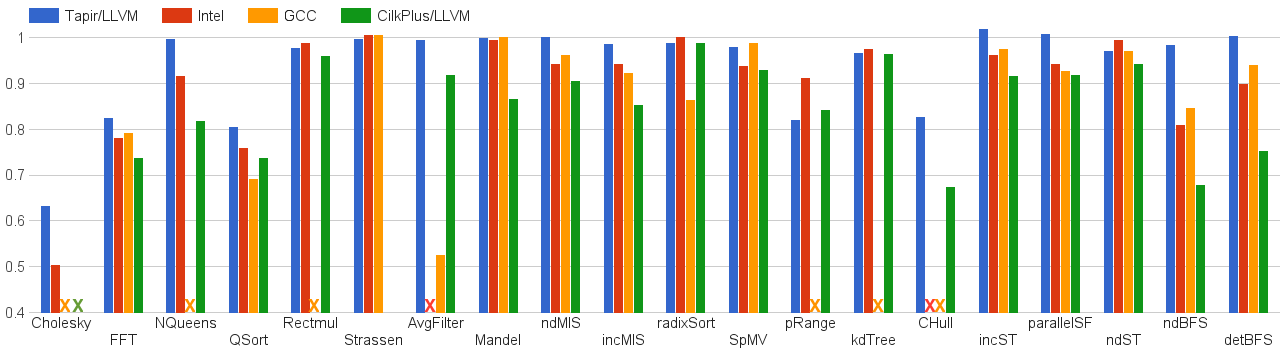
\includegraphics[width=\linewidth]{figures/chart.png}
% \begin{tab}{c}
% \bottomrule
% \end{tab}
% \caption{The work efficiency of mainstream compilers and \tapir/LLVM
%   on the Cilk Plus benchmarks described in \secref{eval}.  For each
%   compiler \tapir/LLVM, ICC 16.0.3, ICC 16.0.3, and GCC 5.3.0, the bar
%   for each benchmark shows the ratio $T_S/T_1$, where the serial
%   running time $T_s$ is running time of the benchmark when the Cilk
%   control constructs are replaced with their serial equivalents, and
%   the $1$-processor running time $T_1$ is the running time of the
%   parallel Cilk code on $1$ processor.  An X means that the compiler
%   failed to compile the code correctly, resulting in a runtime error.}
%   \label{fig:overhead}
% \end{figure*}

This thesis introduces \tapir, a compiler IR that represents logical
fork-join parallelism asymmetrically in the program's CFG\@.  The
asymmetry corresponds to the assumption of \defn{serial semantics}
\cite{FrigoLeRa98}, which means it is always semantically correct to
execute parallel tasks in the same order as an ordinary serial
execution.

\tapir adds three instructions --- \detach, \reattach, and \sync{} ---
to the IR of an ordinary serial compiler to express fork-join parallel
programs with serial semantics.  \subfigref{cfg}{d} illustrates the
\tapir CFG for the \code{fib} function.  As with the symmetric
parallel flow graph in \subfigref{cfg}{c}, \tapir places the logically
parallel recursive calls to \code{fib} in separate basic blocks.  But
these blocks do not join at a synchronization point symmetrically.
Instead, one block connects to the other, reflecting the serial
execution order of the program.

The \tapir approach provides five advantages:
\begin{closeenum}

\item Introducing fork-join parallelism into the compiler is
  relatively easy.

\item The IR is expressive and can represent fork-join control
  constructs from different parallel-language extensions.

\item \tapir parallel constructs harmonize with the invariants
  associated with existing representations of serial code.

\item Standard serial optimizations work on parallel code with few
  modifications.

\item The optimizations enabled by \tapir's parallelism constructs are
  effective in practice.

\end{closeenum}
I discuss each of these advantages in turn.

\section{Ease of implementation}

\tapir's asymmetric representation of logically parallel tasks makes
it relatively simple to integrate \tapir into an existing compiler's
intermediate representation such as LLVM IR~\cite{LLVMLangManual15}.
\figref{loc_breakdown} documents the lines of code added, modified, or
deleted to implement a prototype of \tapir in LLVM\@.  As
\figref{loc_breakdown} shows, \tapir/LLVM was implemented with about
$\fillintheblank{6000}$ lines, compared to LLVM's roughly
$\fillintheblank{4}$-million-line codebase.  Moreover, fewer than
$2000$ lines of code were needed to adapt LLVM's existing compiler
analyses and transformations to accommodate \tapir.

\begin{figure}[h!]
  %\setlength{\tabcolsep}{1pt}
  \small
  \sisetup{group-minimum-digits=4}
  \begin{tab}{lS[table-format=7.0]S[table-format=4.0]@{\hskip -2mm}l}
    \toprule
    \textit{Compiler Component} &
    \textit{LLVM 4.0svn} &
    \multicolumn{2}{l}{\textit{Tapir/LLVM}}
    \\
    \midrule
    Instructions            &  105 995 & 943 &
    \rdelim\}{3}{20pt}[$\num{1 768}$]  \\
    Memory Behavior         &  21 788  & 445 & \hspace{10mm}  \\
    Optimizations           &  152 229 & 380 &   \\
    Parallelism Lowering    &        0 & 3 782 & \\
    % Parallelism Lowering    &        0 & 1 774 & \\
    % New Parallel Optimizations   &        0  & 2 008   \\
    Other                   & 3 803 831  &  460     & \\
    \midrule
    Total                   & 4 083 843  &  6 010 &\\
    \bottomrule
  \end{tab}
  \caption[Code changes required to implement the \tapir/LLVM prototype.]{Breakdown of the lines of code added, modified, or deleted
    in LLVM to implement the \tapir/LLVM prototype.}
  \label{fig:loc_breakdown}
\vspace{-.4cm}
\end{figure}

The breakdown of lines is as follows.  The lines for ``Instructions''
add \tapir's instructions to LLVM IR and adapt LLVM's routines for
reading and writing LLVM IR and bitcode files.  Conceptually, these
changes allow LLVM to correctly compile a \tapir program to a serial
executable with no optimizations.  The lines for ``Memory Behavior''
control how \tapir instructions may interact with memory operations,
preventing the compiler from creating any races.  The lines for
``Optimizations'' perform any adjustments required for LLVM analyses
and transformations to compile a \tapir program at optimization
level~\code{-O3}.  Most of these modifications are not necessary for
creating a correct executable but are added to allow the compiler to
perform additional optimizations, such as parallel tail-recursion
elimination (described in \chapref{opt}).  The lines for ``Parallelism
Lowering'' translate \tapir instructions into Cilk Plus runtime calls
and allow the code to be race-detected with a provably good race
detector~\cite{FengLe99}.  The lines for ``Other'' address a bug in
LLVM's implementation of \code{setjmp} and implement useful features
for our development environment.

% \tbsnote{Technically, it's our own implementation
%   of SP-bags; it's not Cilkscreen:}the Cilk race detector
% Cilkscreen~\cite{Cilkscreen11}.

% Finally, the lines for ``New Parallel Optimizations'' implement new
% optimization passes specifically for parallel code.

\section{Expressiveness of \tapir}

\tapir can express logical fork-join parallelism in parallel programs
that have serial semantics.  For example, \figref{cfg} illustrates how
\tapir can express the parallelism encoded by the \CilkSpawn and
\CilkSync\ linguistics from Cilk++\ \cite{Leiserson10} and Cilk Plus
\cite{IntelCilkPlus10}, as well as the parallelism encoded by OpenMP
\code{task} and \code{taskwait} clauses~\cite{AyguadeCoDu09}.
Similarly, \tapir can express the parallelism encoded by OpenMP
parallel sections~\cite{OpenMP13} and Habanero's \code{async} and
\code{finish} constructs~\cite{CaveZhSh11}.  \tapir can also express
parallel loops, including \CilkFor loops and OpenMP parallel loops
that have serial semantics (described in \chapref{newir}).  Other
parallel constructs, such as those proposed in the C++17 parallelism extensions,
can be represented as well. However, parallel
operations that cannot be expressed in terms of fork-join parallelism,
such as OpenMP's \code{ordered} clause, cannot be represented directly
using \tapir's \detach, \reattach, and \sync instructions.

\tapir makes minimal assumptions about the consistency \cite{Pugh99,
  BoehmAd08} of concurrent memory accesses.  \tapir assumes that
memory is shared among parallel tasks and that virtual-register state
is local to each task.  Parallel instructions in \tapir can exhibit a
\defn{determinacy race}\footnote{Determinacy races are also called
  general races \cite{NetzerMi92} and are distinct from data races,
  which involve nonatomic accesses to critical regions.}
\cite{FengLe99} if they access the same memory location concurrently
and at least one instruction writes to that location.  \tapir itself
does not fully define the possible outcomes of a determinacy race, and
instead defers to existing compiler mechanisms, such as LLVM's atomic
memory-ordering constraints \cite{LLVMLangManual15}, to define
whichever memory model they choose.  For any targeted runtime system,
\tapir relies on a correct implementation of lowering in order to
implement the necessary synchronization, but \tapir is oblivious to
how that runtime system implements the synchronization.

\section{Serial semantics}

By grounding its model of parallelism in serial semantics, \tapir
enables common compiler optimizations for serial code to work on
parallel code.  Intuitively, because \tapir always allows parallel
tasks to execute in their ordinary serial execution order, the
compiler can to optimize parallel code in any manner that preserves
the serial semantics of the program and does not introduce new
determinacy races.  These mild constraints support common
optimizations on parallel code, such as sequentialization, which can
be invalid under models of parallelism without serial
semantics~\cite{VafeiadisBaCh15}.

\section{Optimizations}

In practice, the \tapir team has found that \tapir enables a wide variety of
standard compiler optimizations to work with parallel code.  The
prototype implementation of \tapir/LLVM, for example, successfully
moves the call to \code{norm} in \figref{normalize} outside of the
loop, just as it would for a serial \code{for} loop.  As \chapref{opt}
discusses, \tapir enables other optimizations, including
common-subexpression elimination \cite[Sec.~12.2]{Muchnick97},
loop-invariant-code motion \cite[Sec.~13.2]{Muchnick97}, and
tail-recursion elimination \cite[Sec.~15.1]{Muchnick97}, to work on
parallel code.  \tapir also enables new optimizations on parallel
control flow.

\begin{figure*}[t]
\begin{tab}{c}

\toprule
\end{tab}
  \begin{flushleft}
      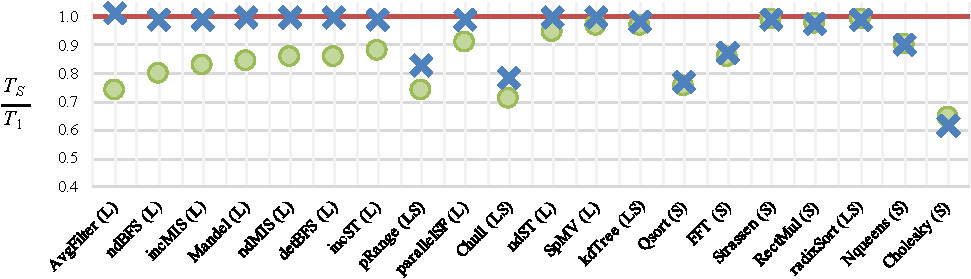
\includegraphics[width=\linewidth]{figures/workeff_scatter.pdf}
  \end{flushleft}
  \vspace*{-5mm}
  \begin{tab}{c}
  \bottomrule
 \end{tab}
 \caption[Graph of work efficiency comparison between Reference and Tapir/LLVM.]{Comparison of the work efficiency of
   \protect\fillintheblank{20} parallel application benchmarks
   compiled using \tapir/LLVM (X's) and the comparable Reference
   compiler (O's), described in \chapref{eval}, which lowers
   parallelism in the compiler front end.  Each point plots the work
   efficiency $T_S/T_1$ of a compiled benchmark, where $T_1$ is the
   work of the benchmark and $T_s$ is the running time of the serial
   elision of the benchmark.  Higher values indicate better work
   efficiency.  The horizontal line at $1.0$ plots the theoretically
   maximum work efficiency $T_S/T_1 = 1$.  Benchmarks are sorted by
   decreasing difference in work efficiency between \tapir/LLVM- and
   Reference-compiled executables.  Benchmarks marked with an ``L''
   use parallel loops, and benchmarks marked with an ``S'' use
   \CilkSpawn.}
  \label{fig:work_efficiency}
\end{figure*}

\section{Evaluation of \tapirllvm}

The compiler optimizations that \tapir enables are effective in
practice.  We evaluated the \tapir approach by measuring the
performance of \fillintheblank{20} Cilk application benchmarks
compiled using \tapirllvm.  We compared the performance of these
executables to those produced by a comparable reference compiler,
called Reference.  Conceptually, Reference lowers parallel linguistic
constructs directly into runtime calls, as mainstream compilers do
today, but otherwise performs the same set of optimization passes as
\tapirllvm.  \chapref{eval} describes our experimental setup in detail,
including the design of Reference.

\figref{work_efficiency} presents the results of comparing \tapirllvm
and Reference in terms of the ``work efficiency'' of the compiled
benchmarks.  To perform this comparison, We compiled each benchmark
using each compiler and then ran the executable on a single processing
core of a multicore machine to measure its \defn{work}, the $1$-core
running time, denoted~$T_1$.  We also used each compiler to compile,
run, and measure the $1$-core running time of the \defn{serial
  elision} \cite{FrigoLeRa98} of each benchmark, denoted $T_S$, in
which the benchmark is converted into a corresponding serial program
by replacing all parallel linguistic constructs with their serial
equivalents.  We then computed the \defn{work efficiency} of each
compiled benchmark, which is the ratio $T_S/T_1$ of the running time
$T_S$ of the benchmark's serial elision divided by the work $T_!$ of
the benchmark.  In theory, the maximum possible work efficiency is
$T_S/T_1 = 1$, but in practice, quirky behaviors of the compiler and
multicore architecture can occasionally produce work efficiencies
greater than~$1$.  As \figref{work_efficiency} shows, for most
benchmarks, the executables compiled using \tapir/LLVM achieve equal
or higher work efficiency than those compiled using Reference.
Moreover, for many benchmarks, and particularly those implemented
using parallel loops, \tapir/LLVM produces executables that achieve
nearly optimal work efficiency.  \chapref{eval} elaborates on these
experiments.

% \tbsnote{I feel the following assessment undersells our results a bit.
%   We should have some more space to expand the discussion of
%   results.}As \figref{work_efficiency} shows, across nearly all of the
% benchmark programs, \tapirllvm produces executables with equal or
% higher work efficiency than the Reference pipeline, validating the
% \tapir approach.

\section{Contributions} 

This thesis makes the following research contributions:
\begin{closeitemize}

\item The design of a compiler IR that represents fork-join
  parallelism asymmetrically, which enables existing serial
  optimizations to operate on parallel code and which also enables
  parallel optimizations.

\item The implementation of \tapir/LLVM in the LLVM compiler by
  modifying about $\fillintheblank{6000}$ source lines of code
  ($\fillintheblank{0.15\%}$ of the $4$-million-line LLVM codebase).

\item The implementation of parallel optimizations such as unnecessary
  synchronization elimination and parallel-loop scheduling.

\item Experiments that demonstrate the advantage of embedding
  fork-join parallelism into a compiler's IR, as opposed to dealing
  with parallelism only in the compiler's front end.

\end{closeitemize}


\section{Outline}

The remainder of this thesis is organized as follows.  \chapref{newir}
describes \tapir's representation and properties.  \chapref{analyses}
discusses how analysis passes can be adapted to operate on \tapir
programs.  \chapref{opt} describes various optimizations on parallel
control flow that \tapir enables.  \chapref{aux} describes auxiliary
software we developed to exercise and test \tapir/LLVM\@.
\chapref{eval} discusses our evaluation of the effectiveness of \tapir.
\chapref{related} discusses related work.  \chapref{concl} provides some
concluding remarks.  An appendix describes how to set up \tapir/LLVM
and how to download and run our suite of application benchmarks.

\chapput{newir}{Tapir}

This chapter describes how \tapir represents logically parallel tasks
asymmetrically in the CFG of a program.  I define \tapir's three new
instructions and how they interact with LLVM's static
single-assignment (SSA) form~\cite[Sec.~6.2.4]{AhoLaSe06}.  Although
I describe \tapir as an extension to LLVM IR~\cite{LLVMLangManual15},
the Tapir team sees no reason why other compilers cannot gain similar advantages
from \tapir-like instructions.

Like LLVM IR, \tapir treats a program function as a CFG $G=(V,E,v_0)$,
where
\begin{itemize}

\item the set $V$ of vertices represents the function's \defn{basic
    blocks}: sequences of LLVM instructions, where control flow can
  only enter through the first instruction and leave from the last
  instruction;

\item the set $E$ of edges denote control flow between (basic) blocks;
  and

\item the designated vertex $v_0\in V$ represents the \defn{entry
    point} of the function.

\end{itemize}
%LLVM IR supports a ``RISC'' instruction set with an infinite set of
%register variables, as well as memory.  \tapir assumes that memory is
%shared among all processors but that register state is local to each
%processor.

% LLVM IR also uses \defn{static single-assignment form}~\cite{???}.

\section{\tapir instructions}

\tapir extends LLVM IR with three instructions: \detach, \reattach,
and \sync.  The \detach and \reattach instructions together delineate
logically parallel tasks, and the \sync instruction imposes
synchronization on parallel tasks.  The three instructions have the
following syntax, where $b,c\in V$:
\begin{inparcode}
\code{detach label }$b$\code{, label }$c$\\
\code{reattach label }$c$\\
\code{sync}
\end{inparcode}
The \code{label} keywords indicate that $b$ and $c$ are (labels of)
basic blocks in~$V$.

% Conceptually, the \detach instruction is similar to a function call,
% and the \reattach instruction is similar to a return.  

The \detach and \reattach instructions together delineate a parallel
task as follows.  A \detach instruction terminates the block $a$ that
contains it and takes a \defn{detached} block $b$ and a
\defn{continuation} block $c$ as its arguments.  The \detach
instruction \defn{spawns} the task starting at block $b$, allowing
that task to execute in parallel with block~$c$.  The control-flow
edge $(a,b)\in E$ is a \defn{detach} edge, and the edge $(a,c)\in E$
is a \defn{continue} edge.  A \reattach instruction, meanwhile,
terminates the block $a'$ that contains it and takes a single
\defn{continuation} block $c$ as its argument, inducing a
\defn{reattach} edge $(a',c)\in E$ in the CFG\@.  The \reattach
terminates the task spawned by a preceding \detach instruction with
the same continuation block.  Together, a \detach instruction and
associated \reattach instructions demark the start and end of a
parallel task and indicate that that task can execute in parallel with
their common continuation block.

For the example in \subfigref{cfg}{d}, the \detach in the
\code{if.else} block and the \reattach in the \code{det} block share
the same continuation block \code{cont}.  Together, this \detach and
this \reattach indicate that the \code{det} block is a parallel task
which can execute in parallel with the \code{cont} block.  In general,
a parallel task delineated by \detach and \reattach can consist of
many basic blocks in a single-entry subgraph.

% In a sense, \detach works like a function call to $b$ that resumes at
% $c$ after the subcomputation rooted at $b$ returns, whereas \reattach
% acts like a return.  But unlike a function call and return, $b$ is a
% block within the CFG of the function containing it, rather than a
% different function in the program, and $b$ and $c$ can operate in
% parallel.

% A \detach does not require that $b$ and $c$ execute in
% parallel, but simply allows the runtime system to schedule them for
% parallel execution, if it so desires.

The \detach and \reattach instructions in a CFG obey several
structural properties.  A \reattach instruction $j$
\defn{reattaches} a \detach instruction $i$ if $i$ and $j$ share a
common continuation block and there is a path from the detached block
of $i$ to~$j$.  \tapir assumes that every CFG $G=(V,E,v_0)$ obeys the
following invariants on every \detach instruction $i$ and \reattach
instruction $j$ in~$G$:
\begin{closeenum}

\item A \reattach instruction reattaches exactly one \detach
  instruction.

\item If $j$ reattaches $i$, then every path from $v_0$ to the block
  terminated by $j$ passes through the detach edge of~$i$, that is,
  the detach edge of $i$ \defn{dominates}~$j$.

\item Every path starting from the detached block of $i$ must reach a
  block terminated by a \reattach instruction that reattaches~$i$.

\item If $j$ reattaches $i$ and a path from $i$ to $j$ passes through
  the detach edge of another \detach instruction $i'$, then it must
  also pass through a \reattach instruction $j'$ that reattaches~$i'$.

\item\label{const:acyclic} Every cycle containing a \detach
  instruction $i$ must pass through a \reattach instruction that
  reattaches~$i$.

\item The continuation block of $j$ cannot contain any $\phi$
  instructions~\cite[Sec~6.2.4]{AhoLaSe06}.

\end{closeenum}
These invariants imply that, at runtime, a \detach instruction $i$
with detached block $b$ and continuation block $c$ spawns the
execution of a \defn{detached sub-CFG}, which is the single entry
sub-CFG starting at $b$ induced by all blocks on paths from $b$ to a
\reattach instruction that reattaches~$i$.

% A \detach instruction $i$ that detaches a block $b$ also
% \defn{detaches} the single-entry sub-CFG of the current function
% induced by all blocks on any path from $b$ to a \reattach instruction
% that reattaches~$i$.  The \defn{continuation} of a CFG detached by $i$
% is the continuation block of $i$, which matches the continuation block
% of every \reattach instruction that reattaches~$i$.

% The block $b$ must be a single-entry block for which
% every exit from the sub-CFG reachable from $b$ --- the parallel task
% spawned by $a$ --- is terminated by a \reattach whose continuation $c$
% matches the continuation in the corresponding \detach instruction ---
% the \detach instruction \defn{reattached} by the \reattach.  For each
% such \reattach instruction, the CFG contains the \defn{reattach} edge
% $(b',c)\in E$, where $b'$ is the block terminated by the \reattach.

% Although memory state is shared among all parallel tasks in \tapir,
The dynamic execution of the program organizes memory as a tree of
\defn{parallel contexts}.  A new parallel context is created as a
child of the current context when control enters a function or follows
a detach edge.  When control executes a \reattach instruction or
leaves a function, the context is destroyed and the parent's context
becomes the current context.  An \code{alloca} instruction allocates
shared memory in the current context.

% Future to-do: Show parallel contexts in figures somehow.

The \sync instruction synchronizes tasks spawned within its parallel
context.  At runtime, a \sync instruction dynamically waits for the
set of sub-CFG's detached in the same parallel context or any of its
descendant parallel contexts to reach a \reattach instruction.  In the
\tapir CFG illustrated in \subfigref{cfg}{d}, for example, the \sync
instruction in the \code{cont} block simply waits for the execution of
the \code{det} block to complete.  Unlike \reattach instructions,
\sync instructions are not explicitly associated with \detach
instructions, and they, in fact, can be executed within conditionals.
A \sync instruction $j$ \defn{syncs} a \detach instruction $i$ if $i$
and $j$ belong to the same parallel context and the CFG detached by
$i$ cannot be guaranteed to have completed when $j$ executes.

% The \detach instructions that $j$ might sync correspond to all
% \detach instructions reachable in a reverse traversal of the CFG
% from $j$ that does not pass through another \sync instruction nor
% traverses a detach or a reattach edge.

% Let us return to the \tapir CFG in \subfigref{cfg}{d} and see how
% the three instructions are used to express the logical parallelism
% of the \code{fib} program in \subfigreftwo{cfg}{a}{b}.  The \detach
% instruction terminating the \code{if.else} block in
% \subfigref{cfg}{d} allows blocks \code{det} and \code{cont} to
% execute in parallel.  The \detach instruction thus creates the
% detach edge $(\mbox{\code{if.else}}, \mbox{\code{det}})\in E$ and
% the continue edge
% $(\mbox{\code{if.else}}, \mbox{\code{cont}})\in E$.  The \reattach
% instruction in the \code{det} block reattaches the \detach
% instruction in the \code{if.else} block, terminating the basic block
% \code{det} and creating the reattach edge
% $(\mbox{\code{det}}, \mbox{\code{cont}})\in E$.


\section{Static single-assignment form}

LLVM's static single-assignment (SSA) form
\cite[Sec.~6.2.4]{AhoLaSe06} must be adapted for \tapir programs.  SSA
form ensures that each virtual register is set at most once in a
function.  LLVM IR employs the \defn{$\boldmath \phi$ instruction}
\cite[Sec~6.2.4]{AhoLaSe06} to combine definitions of a variable from
different predecessors of a basic block.  In adapting SSA to \tapir,
one concern is that a $\phi$ instruction might allow registers defined
in the detached sub-CFG to be used in the continuation.  A basic block
containing a $\phi$ instruction must avoid inheriting register
definitions from predecessors that are connected by reattach edges.
Otherwise, a register in the detached sub-CFG might not have been
computed by the time the continuation executes.

We implemented this constraint by simply forbidding reattach edges
from going into basic blocks with $\phi$ instructions.  But what if
the continuation $c$ of a \detach instruction begins with a $\phi$
instruction?  In this case, \tapir creates a new basic block $c'$
containing only a branch instruction to~$c$.  \tapir reroutes the reattach
and continuation edges originally going to $c$ so that they go instead
to~$c'$.  All other edges going to $c$ are left in place.

The reason this solution works is as follows.  No reattach edges in
the resulting CFG go to blocks containing $\phi$ instructions.
Because a detached sub-CFG does not dominate any outside block,
registers in the detached CFG can only be used in $\phi$ instructions
of the immediate successors of the detached sub-CFG\@.  Since the
continuation is the only immediate successor of the detached sub-CFG
and it contains no $\phi$ instructions, no registers from the detached
sub-CFG may be accessed in the continuation.


\section{Asymmetry in \tapir}

% The \detach, \reattach, and \sync instructions exhibit serial
% semantics.  When executed on a single processor, a \detach instruction
% acts like an unconditional branch to its detached block, and a
% \reattach instruction acts like an unconditional branch to its
% continuation block.  The CFG detached by a \detach instruction $d$
% therefore precedes the execution of the continuation block of $d$ in a
% serial execution.  A \sync instruction is therefore a no-op in a
% serial execution.

The \detach and \reattach instructions express parallel tasks
asymmetrically both syntactically in the structure of the CFG and
semantically in the way memory state is managed.  Both asymmetries are
illustrated in \subfigref{cfg}{d}.

First, the CFG detached by a \detach instruction is connected by a
reattach edge to the continuation block of that instruction, even
though they can execute in parallel.  For example, the reattach edge
between \code{det} and \code{cont} in \subfigref{cfg}{d} breaks the
symmetry between them.  Reattach edges reflect the serial semantics of
a \tapir program, which dictates that a serial execution of the
program executes the detached CFG to completion before starting to
execute the continuation block.  In fact, the parallel task delineated
by a \detach and a \reattach instruction can be \defn{serialized} by
replacing the \detach instruction with an unconditional branch to its
detached block and replacing the \reattach with an unconditional
branch to its continuation block.  In contrast, parallel flow graphs
and similar previously explored representations join logically
parallel tasks in the CFG at a synchronization point.  By supporting
separate \reattach and \sync instructions, \tapir decouples the
termination of a parallel task from its synchronization.

% An entire \tapir program can be serialized
% as follows:
% \begin{closeitemize}

% \item Replace every \detach instruction by an unconditional branch to
%   its detached block, which effectively removes the continue edge
%   from~$E$.

% \item Replace every \reattach instruction that reattach a \detach
%   instruction $i$ with an unconditional branch to the continuation
%   block of~$i$.

% \item Remove all \sync instructions.

% \end{closeitemize}
% The resulting program is called the \defn{serial elision}
% \cite{FrigoLeRa98} of the \tapir program, because all the parallelism
% has been elided.  The serial elision contains no \tapir keywords and
% is a serial LLVM program that employs standard LLVM~IR\@.

Second, although memory state is shared among all parallel tasks in
\tapir, a virtual register defined in a detached sub-CFG is not
accessible in its parent parallel context.  For example, the
continuation block \code{cont} in \subfigref{cfg}{d} cannot assume
that the register value \code{x0} returned by \code{fib(n-1)} in block
\code{det} is accessible, because the two basic blocks belong to
different parallel contexts.  Thus, \code{cont} must load it again
after the \sync instruction.

% \tapir adopts LLVM's strategy for virtual register availability.  A
% register defined in a basic block $a$ is only available to subsequent
% instructions in~$a$, but not to instructions before the definition.
% \wmnote{Potentially remove -- task 9}The register is only available
% within a basic block $b$ if $a$ dominates~$b$.  As a result, virtual
% registers defined in a detached sub-CFG are not available across
% reattach edges.  Hence, to communicate data out of a detached sub-CFG,
% the data must be transferred through shared memory and not through
% registers.  In addition to preserving the fundamental invariants of
% LLVM, which simplifies the implementation of \tapir/LLVM, this
% behavior mimics what a runtime system must do more accurately than a
% design in which registers from multiple parallel tasks are all
% available after the tasks join.

% \secref{analyses} shows how \tapir's asymmetric representation makes
% it easy for existing compiler analyses to work with \tapir CFG's.

\begin{figure}[t]
\begin{tab}{c}
\toprule
\end{tab}
\centering{%
  \begin{tikzpicture}
    \node [basic block, label=left:\fccode{entry:}] (entry)
    {\parbox{3.6cm}{\fccode{\fc{k}{br} \fc{p}{(}0 \fc{o}{<} n\fc{p}{)}\fc{p}{,} head\fc{p}{,} exit}}};
    \node [basic block, below= of entry, label=left:\fccode{head:}]
    (head)
    {\fccode{i0 \fc{o}{=} \fc{k}{$\phi$}\fc{p}{(}\fc{p}{[}0\fc{p}{,}entry\fc{p}{]}\fc{p}{,}\fc{p}{[}i1\fc{p}{,}inc\fc{p}{]}\fc{p}{)}}\\
      \textcolor{red}{detach body\fc{p}{,} inc}};
     \node [basic block, below= of head, label=left:\fccode{body:},
     xshift=-1cm] (body)
     {\fccode{norm0 \fc{o}{=} norm\fc{p}{(}in\fc{p}{,}n\fc{p}{)}}\\
       \fccode{out\fc{o}{[}i0\fc{o}{]} \fc{o}{=} in\fc{o}{[}i0\fc{o}{]} \fc{o}{/} norm0}\\
       \textcolor{red}{reattach inc}};
     \node [basic block, below= of body, label=left:\fccode{inc:},
     xshift=1cm] (inc) {
       \fccode{i1 \fc{o}{=} i0 \fc{o}{+} \fc{l+m}{1}}\\
       \fccode{\fc{k}{br} \fc{p}{(}i1 \fc{o}{<} n\fc{p}{)}\fc{p}{,} head\fc{p}{,} exit}};
     \node [basic block, below= of inc, label=left:\fccode{exit:},
     xshift=0cm, align=left] (exit)
     {\parbox{2.6cm}{\textcolor{red}{sync}\\\fccode{\fc{k}{return}}}};
    \path [cfedge]
    (entry) edge node[right] {\small T} (head)
    (head)  edge node [left, xshift=-.05cm] {\small detach} (body)
    (head)  edge[bend left=58] node[right] {\small continue} (inc)
    (body)  edge node[left] {\small reattach} (inc)
    (inc)  edge[bend right=90] node[right] {\small T} (head)
    (inc)  edge[] node[left] {\small F} (exit)
    (entry)  edge[in=0,out=0] node[right] {\small F} (exit);
  \end{tikzpicture}}
\begin{tab}{c}
\bottomrule
\end{tab}
\caption{\tapir CFG for the parallel loops in \figref{normalize}.}
  \label{fig:tapir_normalize}
\end{figure}

\section{Parallel loops in \tapir}

\figref{tapir_normalize} illustrates \tapir's default representation
of the parallel loops from \figref{normalize}.  As
\figref{tapir_normalize} shows, \tapir can represent a parallel loop
in the CFG as an ordinary loop, where the \code{head} block repeatedly
spawns the \code{body} block, and the \code{exit} block syncs the
detached CFG's.  \chapref{opt} describes how this representation of
parallel loops allows existing compiler loop optimizations to operate
on \tapir parallel loops with only minor modifications.  Although this
loop structure can exhibit poor parallel performance when the loop
body is small, separate optimization passes in \tapir/\mbox{LLVM} (see
\chapref{opt}) transform this parallel-loop representation into a
divide-and-conquer form that exhibits good performance.


%%% Local Variables:
%%% mode: latex
%%% TeX-master: "tapir"
%%% End:

%  LocalWords:  LLVM multithreading multicore OpenMP Cilk GCC Cilk's
%  LocalWords:  pseudocode metadata LLVM's bitcode codebase CFG's CFG
%  LocalWords:  subexpression interleavings subcomputations runtime
%  LocalWords:  vertices subcomputation OpenMP's

\chapput{analyses}{Analysis passes}

This chapter describes how LLVM's analysis passes can be adapted to
operate on \tapir programs.  I first discuss constraints on how
\tapir programs can be safely transformed.  Implementing these
contraints on LLVM optimization passes primarily involves adapting
standard compiler analyses --- specifically alias analysis
\cite[Ch.~12]{AhoLaSe06}, dominator analysis \cite[Ch.~9]{AhoLaSe06},
and data-flow analysis \cite[Ch.~9]{AhoLaSe06} --- to accomodate
\tapir's instructions.  I describe how each of these analyses was
minimally modified to support \tapir.

\section{Constraints on transformations}

% Because \tapir allows for parallel execution, rather than demand it,
% many common compiler optimizations for serial programs can operate
% across \tapir's instructions.

To be correct, a code transformation on a \tapir program must preserve
the program's serial semantics, and it must not introduce any new
behaviors into the program's set of behaviors.  A program can exhibit
more than one behavior if it contains a determinacy race.  In general,
the result of a determinacy race can vary nondeterministically from
run to run depending on the order in which the participating
instructions access the memory location.  To avoid introducing new
behaviors, code transformations must not create determinacy races,
although they can eliminate determinacy races.  Many existing serial
optimizations can be adapted to respect these properties by adapting
the standard compiler analyses they rely on.  I now describe how
LLVM's alias, dominator, and data-flow analyses were
adapted for \tapir.

% One way a code transformation can preserve the two correctness
% properties is by \defn{serializing} a portion of the CFG: constraining
% parallel tasks to execute in the serial-execution order, rather than
% allowing the runtime system to order things as it sees fit.
% \tbsnote{The following description of serialization feels out of place
%   to me.  It might fit better with the discussion on the asymmetry of
%   \tapir's representation.}

\section{Alias analysis}

% Key to optimizing \tapir programs correctly is preventing code-motion
% optimizations from introducing determinacy races.  For example, if two
% instructions access the same memory location and one of them writes to
% that location, a transformation should not move these instructions to
% execute in parallel if originally they were guaranteed to execute in
% series.

LLVM uses alias analysis \cite[Ch.~12]{AhoLaSe06} to determine whether
different instructions might reference the same locations in memory,
and in particular, to restrict the reordering of instructions that
access the same memory.  \tapir/LLVM modifies LLVM's alias analysis to
prevent optimizations that move code around from introducing
determinacy races.  In particular, \tapir adapts LLVM's alias analysis
to treat the instructions as if they access memory.  For example,
consider an instruction $k$ that performs a load or a store.  There
are four cases to consider when moving $k$ around either a \detach
instruction $i$ or a \sync instruction~$j$:
\begin{closeenum}

\item\label{case:after_detach} The instruction $k$ moves from before
  $i$ to after~$i$.

\item\label{case:before_detach} The instruction $k$ moves from after
  $i$ to before~$i$.

\item\label{case:after_sync} The instruction $k$ moves from before $j$
  to after~$j$.

\item\label{case:before_sync} The instruction $k$ moves from after $j$
  to before~$j$.

\end{closeenum}
Neither \caseref{before_detach} nor \caseref{after_sync} can introduce
a determinacy race, because both motions serialize the execution of
$k$ with respect to the sub-CFG detached by~$i$.
\casereftwo{after_detach}{before_sync} might introduce a determinacy
race, however, if $k$ loads or stores a memory location that is also
accessed by the CFG detached by~$i$.  To handle
\caseref{after_detach}, $i$ is treated as if it were a function call
that accesses all memory locations accessed in the CFG detached
by~$i$.  Similarly, for \caseref{before_sync}, $j$ is treated as if it
were a function call that accesses all memory locations accessed by
all instructions that $j$ might sync.  A \code{reattach} instruction
is treated as a compiler fence that prevents instructions from moving
across it.  With these modifications, existing rules in LLVM that
restrict reordering of loads and stores properly restrict memory
reordering around \tapir's instructions.


\section{Dominator analysis}

Optimization passes determine what values are available to an
instruction in part by using dominator analysis
\cite[Ch.~9]{AhoLaSe06}, which deduces the dominance relation between
all basic blocks and edges in a CFG\@.  To handle \tapir programs
correctly, optimization passes must not mistakenly cause instructions
to use virtual registers that are defined in logically parallel tasks.
If instruction $i$ dominates instruction $j$, than an optimization
pass might assume that the value produced by $i$ is always available
when $j$ executes.

% determine that one instruction is guaranteed to execute
% before another when \tapir allows those instructions to execute in
% parallel.  Existing optimization determine when one instruction is
% guaranteed to execute before another using 

% Many optimization passes must determine what basic blocks or
% control-flow edges in a CFG dominate a particular point in the
% CFG\@.

The asymmetry of \tapir's representation allows LLVM's dominator
analysis to analyze \tapir programs correctly without any changes.
Ignoring the names of edges, the difference between the CFG
$G=(V,E,v_0)$ of a \tapir program and the CFG $G'=(V,E',v_0)$ of its
serial elision is the set $E-E'$ of continue edges, each of which
connects a \detach instruction to its continuation.  A continue edge
short-cuts a detached sub-CFG, changing the continuation's immediate
dominator from the detached sub-CFG to the block containing the
\detach instruction itself.  This configuration of detach, reattach,
and continue edges looks much like an ordinary \code{if} construct in
which the detached sub-CFG is conditionally executed.  As a result,
dominator analysis never concludes that an instruction in a detached
sub-CFG can execute before the corresponding continuation block.

% \tbsnote{The story with postdominator analysis seems murkier to me.}

% LLVM's dominator analysis requires no changes to handle \tapir
% programs.


\section{Data-flow analysis}

A wide class of code transformations, including those that might move
instructions across a reattach edge, rely on data-flow analysis
\cite[Ch.~9]{AhoLaSe06} to examine the propagation of values along
different paths through a CFG $G=(V,E,v_0)$.  Fundamental to data-flow
analysis is an understanding of the set of possible program states at
the beginning and end of each basic block $b\in V$, denoted
$\proc{in}(b)$ and $\proc{out}(b)$, respectively.

To illustrate how LLVM's data-flow analyses were adapted to \tapir,
let us examine the particular case of forward data-flow analysis.
(Backward data-flow analysis is similar.)  In an ordinary serial CFG,
forward data-flow analysis evaluates $\proc{in}(b)$ as the union of
$\proc{out}(a)$ for each predecessor block $a$ of $b$:
\[
\proc{in}(b) = \bigcup_{(a,b)\in E}\proc{out}(a)\ .
\]

To handle \tapir CFG's, data-flow analyses must be adapted
specifically to handle reattach edges.  Because \tapir's asymmetric
representation propagates virtual registers and memory state
differently across a reattach edge, the modifications to LLVM data
analyses consider registers and memory separately.

For variables stored in shared memory, the
standard data-flow equations remain unchanged. Thus, LLVM need not be
modified to handle them for \tapir.

For register variables, however, LLVM's data-flow analyses must be
modified to exclude the values in registers from an immediate
predecessor $a$ of a basic block $b$ if the edge $(a,b)\in E$ is a
reattach edge.  Denote the set of reattach edges in $E$ by~$E_{R}$.
For a \tapir CFG, forward data-flow analyses define $\proc{in}(b)$ for
register variables as
\[
\proc{in}(b) = \bigcup_{(a,b)\in E - E_{R}}\proc{out}(a)\ ,
\]
that is, they ignore predecessors across a reattach edge.  With this
change, \tapir/LLVM correctly propagates register variables through
the CFG, never allowing register values in a basic block to use
register values set in a logically parallel detached sub-CFG.

% Data-flow analyses on memory values are generally adapted to \tapir
% programs by handling the incoming values $\proc{in}(c)$ to a
% continuation block $c$ for a memory location $\ell$ in a special
% manner.  Let $d$ and $r$ be predecessors of $c$ where $d$ is
% terminated by a \detach instruction $i$ and $r$ is terminated by a
% \reattach instruction that reattaches~$i$.  If data-flow analysis
% finds that $\proc{out}(d)$ and $\proc{out}(r)$ are not the same for
% memory location $\ell$, then the value of $\ell$ is not deterministic
% at the start of~$c$.  In this case, it is safe for data-flow analyses
% to assume the most conservative value for $\ell$ at the start of~$c$.

% Although optimizations on memory must be handled carefully to
% interoperate with \tapir, only a limited set of optimizations in LLVM
% that operate on memory values, because these values must be explicitly
% loaded into and stored from register variables.


% Excluding the restriction that
% registers from \reattach predecessors may not be used in the continuation,
% this additional constraint is no less expressive than the scenario where
% $\phi$ nodes were permitted in the the sucessors of \reattach edges.
% 
% This is because you can always construct a CFG that does not have $\phi$
% nodes in the sucessors of \reattach edges from a CFG which does have
% $\phi$ nodes in the successors of \reattach edges and does not use
% values from the detached sub-CFG in the continuation.
% 
% For example, suppose the continuation $c$ that has a $\phi$ node. Split it
% into two blocks $a$ and $b$. The block $a$ contains only a branch to 
% $b$ and contains the reattach edge and detach edge as predecessors. The block $b$
% contains all the instructions of $c$, including $\phi$ nodes, and all other
% predecessors branch to $b$.

%%% Local Variables:
%%% mode: latex
%%% TeX-master: "tapir"
%%% End:

%  LocalWords:  LLVM multithreading multicore OpenMP Cilk GCC Cilk's
%  LocalWords:  pseudocode metadata LLVM's bitcode codebase CFG's CFG
%  LocalWords:  subexpression interleavings subcomputations runtime
%  LocalWords:  vertices subcomputation OpenMP's nonatomic dominator
%  LocalWords:  nondeterministically nondeterministic postdominator
%  LocalWords:  dominators postdominators


\chapput{opt}{Optimization passes}

\tapir enables LLVM's existing optimization passes
\cite{LLVMPassesManual15} to work across parallel control flow.  It
also enables new optimization passes that specifically target \tapir's
fork-join parallel constructs.  This chapter discusses four
representative optimizations.  Common-subexpression elimination\
\cite[Sec.~12.2]{Muchnick97} illustrates an optimization pass that
``just works'' with the additional \tapir instructions.
Loop-invariant code motion\ \cite[Sec.~13.2]{Muchnick97}, and
tail-recursion elimination\ \cite[Sec.~15.1]{Muchnick97} were the only
two out of LLVM's roughly $80$ optimization passes that required any
modification to work effectively on parallel code.  Parallel-loop
scheduling serves as an example of a new optimization pass.

% \tbsnote{Discuss parallel-specific opts as well?  Discuss work-span
%   analysis?}

%To collect the performance measurements described in this section, we
%ran microbenchmark tests using our modified LLVM compiler.  We ran
%these tests on Amazon AWS \code{c4.8xlarge} spot instances, which
%contain a dual-socket Intel Xeon E5-2666 v3 system with a total of
%\SI{60}{\gibi\byte} of memory.  Each Xeon is a $2.9$\,GHz $18$-core
%CPU with a shared \SI{25}{\mebi\byte} L3-cache.  Each processor core
%has a \SI{32}{\kibi\byte} private L1-data-cache and a
%\SI{256}{\kibi\byte} private L2-cache.  In general, microbenchmarks
%were compiled using \code{-O3} optimizations, excluding the
%targeted optimization.

\section{Common-subexpression elimination}


\begin{figure}[t]
  \begin{tabular*}{\linewidth}{@{\extracolsep{\fill}}l@{}l}
    \begin{minipage}[T]{.45\linewidth}
        \subfiglabel{a}
      \begin{flushleft}
        \ccodefig{figures/search}
      \end{flushleft}
        \vspace{1ex}
    \end{minipage}
    &
    \begin{minipage}[T]{.45\linewidth}
    \subfiglabel{b}
      \begin{flushleft}
        \ccodefig{figures/search_cse}
      \end{flushleft}
      \vspace{0.1ex}
    \end{minipage}
  \end{tabular*}
  \caption[Example of common-subexpression elimination on a Cilk
    program.]{Example of common-subexpression elimination on a Cilk
    program.  \subfigcap{a}~The function \code{search}, which uses
    parallel divide-and-conquer to apply the function
    \code{search_base} to every integer in the closed interval
    [\code{low}, \code{high}].  \subfigcap{b}~An optimized version of
    \code{search}, where the common subexpression \code{(low+high)/2}
    in \lireftwo{search_expr}{search_dupexpr} of the original version
    is computed only once and stored in the variable \code{mid} in
    \liref{search_cse_call} of the optimized version.}
  \label{fig:search}
\end{figure}

The common-subexpression elimination (CSE) optimization identifies
redundant calculations and transforms the code so that they are only
computed once.  For example, the expression \code{(low+high)/2} in
\subfigref{search}{a} is computed in both \liref{search_expr} and
\liref{search_dupexpr}.  \tapir/LLVM performs CSE on this code,
producing code equivalent to that in \subfigref{search}{b}.  Existing
mainstream compilers that support fork-join parallelism do not
eliminate this common subexpression, however, and they compute
\code{(low+high)/2} twice.  \tapir/LLVM can perform CSE across either
a continue edge, as in the example, or a detach edge.  Like the vast
majority of optimization passes in \tapir/LLVM, CSE ``just works'' on
\tapir code without any modifications to LLVM's CSE pass.

\section{Loop-invariant code motion}

The loop-invariant code motion (LICM) optimization
\cite[Sec.~13.2]{Muchnick97} aims to move computations out of loop
bodies if they compute the same value on every iteration of the loop.
LICM is responsible, for example, for moving the call to \code{norm}
in the parallel loop in \subfigref{normalize}{a} outside of the loop,
as described in \chapref{intro}.  By adapting LICM to handle parallel
loops, \tapir/LLVM reduces the asymptotic serial running time of this
parallel loop from $\Theta(n^2)$
to~$\Theta(n)$.

% Indeed, we observe in practice that doubling the size $n$ of the
% vectors increases the running time 

% \begin{tabular*}{\textwidth}{ c|c|c|c|c }
%               & N=40K,T=1 & N=40K,T=36 & N=80K,T=1 & N=80K,T=36\\
% \hline
% \tapir O3     &   0.09  &  0.12 &   0.19  &   0.23 \\
% No Opt        & 215.60  & 29.63 & 863.01  & 108.06
% \end{tabular*}

\tapir/LLVM requires a minor change to LLVM's LICM pass to handle
parallel loops.  Consider the CFG illustrated in
\figref{tapir_normalize}, which models the parallel loops in
\figref{normalize}.  For the serial elision of the loop, which would
have a similar graph structure except with the continue edge missing,
LLVM attempts to find candidate computations to move outside the loop
by looking for instructions in the basic blocks of the loop body that
dominate the exit block of the loop, such as the block \code{inc} in
\figref{tapir_normalize}.  (The block labeled \code{exit} is the exit
of the function, not the loop exit.)  For a parallel loop, however,
this analysis fails to identify any code to move due to the existence
of the continue edge.  As \figref{tapir_normalize} shows, with the
continue edge, blocks in the loop body can never dominate the exit
block \code{inc} as they could for the serial elision.

\tapir/LLVM modifies LLVM's LICM pass to handle a parallel loop by
analyzing the serial elision of the loop, which essentially means
ignoring continue edges.  For simple parallel loop structures with a
single continue edge, such as that shown in \figref{tapir_normalize},
this modification is implemented by finding blocks in the loop body
that dominate the predecessors of the loop exit.  The modification
required changing only \fillintheblank{$25$} lines of LLVM's LICM
pass.

%\section{Scalar replacement of aggregates}

%The scalar-replacement-of-aggregates optimization (SROA) attempts to
%find structures and arrays in a program in a function and store their
%individual fields in register variables.  Typically, because a whole
%structure or array is too large to store in a register, such variables
%are stored in memory instead.  SROA can therefore reduce the number of
%memory accesses a function performs, thereby improving performance.

%Without modifying SROA beyond the changes discussed in \secref{eval},
%LLVM can perform SROA on \tapir programs.  We found that LLVM performs
%SROA on the \tapir representation of a Cilk program from the Cilk-5
%benchmark suite\ \cite{FrigoLeRa98} that computes a sparse Cholesky
%decomposition.  This program uses a quad tree data structure to manage
%the blocks within a matrix.  The traditional compilation method of
%translating Cilk parallel lingustics to runtime calls, meanwhile,
%prevents LLVM from performing SROA on the quad-tree data structure in
%this program.  For this program, optimizing the \tapir representation
%reduces the number of cache references in the serial execution by
%\fillintheblank{$13\percent$--$20\percent$} and improves the serial
%running time of the program by
%\fillintheblank{$15\percent$--$24\percent$}, depending on optimization
%level.

% \tbsnote{\code{CILK_NWORKERS=1 ./cholesky -n 2000 -z 16000}}


\section{Tail-recursion elimination}

\begin{figure}[t]
  \begin{tabular*}{\linewidth}{@{\extracolsep{\fill}}l@{}l}
    \begin{minipage}[T]{.45\linewidth}
    \subfiglabel{a}
      \begin{flushleft}
        \ccodefig{figures/pqsort}
      \end{flushleft}
        \vspace{1ex}
        \subfiglabel{c}
      \begin{flushleft}
        \ccodefig{figures/pqsort_tre}
      \end{flushleft}
      \vspace{0.1ex}
    \end{minipage}
    &
    \begin{minipage}[T]{.45\linewidth}
    \subfiglabel{b}
      \begin{flushleft}
        \ccodefig{figures/pqsort_inl}
      \end{flushleft}
    \end{minipage}
    \vspace{1ex}\\
  \end{tabular*}
  \caption[Example of tail-recursion elimination on a parallel
    quicksort program.]{Example of tail-recursion elimination on a parallel
    quicksort program.  \subfigcap{a}~The Cilk function \code{pqsort}
    sorts an array of integers in the range specified by the
    \code{start} and \code{end} pointers.  \subfigcap{b}~A version of
    \code{pqsort} where the recursive tail call on
    \liref{pqsort_tail_call} has been replaced by one round of
    inlining.  \subfigcap{c}~A version of \code{pqsort} where
    tail-recursion elimination has removed the recursive tail call on
    \liref{pqsort_tail_call}.}
  \label{fig:pqsort}
\end{figure}

Tail-recursion elimination (TRE) \cite[Sec.~15.1]{Muchnick97} aims
to replace a recursive call at the end of a function with a branch to
the start of the function.  By eliminating these recursive tail calls,
TRE can avoid function-call overheads and reduce the stack space they
consume.  This optimization can especially benefit fork-join parallel
programs, as many parallel runtime systems impose additional setup and
cleanup overhead on a spawned function.
%  A common efficient
%implementation of parallel loops, for example, spawns the parallel
%loop iterations using recursive
%divide-and-conquer~\cite[Sec.~8.3]{McCoolRoRe12}.  Work-stealing
%running times, moreover, often use additional data structures per
%function to manage logically parallel tasks~\cite{FrigoLeRa98,
%  LeeBoHu10}.

LLVM's existing TRE pass can perform the TRE optimization on \tapir
programs with just a minor modification.  Specifically, the modified
TRE pass ignores \sync instructions after the tail-recursive call.
Further, if TRE is applied and ignores a \sync instruction, it must
then insert a \sync instruction before any remaining returns.  This
modification to LLVM's TRE pass required changing only
\fillintheblank{$68$} lines.

To see why these \sync instructions can be safely ignored, consider
\figref{pqsort}, which illustrates how \tapir/LLVM's TRE pass operates
on the \code{pqsort} function, a parallel version of Hoare's quicksort
algorithm~\cite{Hoare61}.  The original tail-recursive code is shown
in \subfigref{pqsort}{a}.  \subfigref{pqsort}{b} illustrates the
result of simply inlining the tail-recursive call.  For the inlined
code, all \code{return} statements are replaced with branches to the
\code{join} label.  Because there is a \CilkSync at the start of
\code{join}, the \CilkSync on \liref{inlined_sync} can be eliminated.
call an arbitrary number of times, TRE can safely ignore a \CilkSync
instruction after the final tail-recursive call, assuming that it
inserts a \CilkSync instruction before all remaining returns.

\section{Parallel-loop scheduling and lowering}

As discussed above and in \chapref{newir}, Tapir effectively represents
a parallel loop as a serial loop over a body that is spawned every
iteration.  Depending on the number of iterations of the loop and the
amount of work inside each loop, however, statically scheduling loop
iterations in this way may be inefficient.  For a parallel loop with a
large number of iterations, for instance, it is faster to schedule the
iterations in a recursive divide-and-conquer fashion, which produces
more parallelism (see \cite[Sec.~8.3]{McCoolRoRe12}.
For parallel loops with few iterations, however, the additional
function calls required to perform the parallel divide-and-conquer can
make the loop run slower than simply spawning off the iterations.

\tapir/LLVM implements a parallel optimization pass that schedules the
iterations of a parallel loop using recursive divide-and-conquer, but
only if that loop contains sufficiently many iterations.  This pass is
implemented as part of \tapir/LLVM's \fillintheblank{$3800$}-line
lowering pass, which translates \detach, \reattach, and \sync
instructions into appropriate Cilk Plus runtime
calls~\cite{IntelCilkPlusABI10}.  In particular, \tapir/LLVM uses the
Cilk Plus runtime calls for \CilkFor loops
\cite[Sec~10.7]{IntelCilkPlusABI10} to schedule parallel
loops.  % We could have separated parallel-loop scheduling from
% lowering by having the parallel-loop-scheduling pass directly emit the
% appropriate function to schedule a parallel loop using
% divide-and-conquer.
Although we could have separated parallel-loop scheduling from
lowering, we chose to combine these two passes so that we could
perform fair comparisons between \tapir/LLVM and compilers that lower
parallel constructs in their front end.  We plan to separate the
parallel-loop-scheduling and lowering passes in a future version of
\tapir/LLVM\@.

% The lowering pass translates \detach, \reattach, and \sync
% instructions into appropriate Cilk Plus runtime
% calls~\cite{IntelCilkPlusABI10}.  This pass lifts detached CFG's in
% the program into helper functions and inserts Cilk runtime calls to
% allow those helper functions to run in parallel.  This pass, which
% amounted to approximately \fillintheblank{$1900$} lines, allowed us to
% run codes compiled with \tapir to verify that parallel executions
% produce correct results.

% \tapir/LLVM implements a pass that schedules a parallel loop using
% Cilk's runtime-system method for \CilkFor loops
% \cite[Sec.~10.7]{IntelCilkPlusABI10} only if that loop contains a
% sufficient number of iterations.
% % \tapir/LLVM implements a new optimization pass that transforms
% % parallel loops into divide-and-conquer parallel loops, but only if
% % there are sufficient iterations.
% This pass was implemented in \fillintheblank{approximately $2000$}
% lines of code, some of which is devoted to producing a parallel-loop
% report for the programmer.

%\wmnote{should there be a figure here?}

\section{Other optimization passes}

\tapir/LLVM implements two minor parallel optimization passes:
unnecessary-synchronization elimination and puny-task elimination.
\defn{Unnecessary-synchronization elimination} identifies and
eliminates \sync instructions that could not possibly sync a detached
sub-CFG\@.  \defn{Puny-task elimination} serializes detached sub-CFG's
that perform little or no work.  If the runtime overhead of creating a
parallel task outweighs the work in the task, the task might as well
be run serially.  Both of these optimization passes were implemented
in \fillintheblank{$52$} lines of code by augmenting LLVM's
SimplifyCFG pass.

%%% Local Variables:
%%% mode: latex
%%% TeX-master: "tapir"
%%% End:

%  LocalWords:  LLVM multithreading multicore OpenMP Cilk GCC Cilk's
%  LocalWords:  pseudocode metadata LLVM's bitcode codebase CFG's CFG
%  LocalWords:  subexpression interleavings subcomputations runtime
%  LocalWords:  vertices subcomputation OpenMP's inlining quicksort
%  LocalWords:  CSE LICM TRE inlined Hoare's

%\chapput{popt}{Parallel optimization passes}


\section{Synchronization Elimination}

TODO

\section{Small Task Serialization}

TODO

\section{Parallel Loop Indexing}

TODO

\section{Coarsening}


\section{Parallel Loop Fusion}
Interestingly, in addition to both permitting serial optimizations to operate on parallel code and allowing optimizations on the parallel 


\section{Non-deterministic LICM}
\begin{verbatim}
__attribute__((const))
int Object::method1();

void Object::method2(int cnt);

Object* obj = ...;
cilk_for() {
  int cnt = obj->method1();
  obj->method2(cnt);
}

\end{verbatim}

\begin{verbatim}
__attribute__((const))
int method1(int* obj);

void method2(int* obj);

int* obj;
cilk_for() {
  int cnt = method1(obj);
  method2(obj);
}


#define cilk_for _Cilk_for

__attribute__((const))
int method1(int* obj);

void method2(int* obj, int cnt);

int* acq();

int len();

int main() {
  int n = len();
  int* obj = acq();


  cilk_for(int i=0; i<n; i++) {
    int cnt = method1(obj);
    method2(obj,cnt);
  }

}
\end{verbatim}

\section{Interplay optimizations (Spawn unswitching)}

Or perhaps task sinking
\begin{verbatim}
cilk_spawn {
    if (value) {
        foo(i);
    }
}

becomes

if (value) {
    cilk_spawn {
        foo(i);
    }
}
\end{verbatim}





\chapput{aux}{Auxiliary software}

This chapter describes auxiliary software that the Tapir team developed to
exercise and test \tapir/LLVM\@.  Although our research focuses on the
middle end of the compiler, we implemented a front end for Cilk Plus.
In addition, we developed compiler instrumentation that allows the
compiler to interface to a race detector to verify the correctness of
the \tapir/LLVM implementation.

% and a pass to lower \tapir constructs to Intel Cilk Plus runtime calls

To create the front end, the Tapir team created a modification of the Clang front
end called PClang, which translates Cilk Plus codes to \tapir.  We
also created a version of Clang that can handle some OpenMP codes.
PClang handles most of the fork-join control constructs specified by
the Cilk Plus programming model, and specifically, enough to run all
the benchmarks described in \chapref{eval}.

We augmented \tapir/LLVM in two ways to test the correctness of the
implementation.  First, we modified LLVM's internal verification pass
to check that \tapir's invariants are also maintained.  Second, we
added an instrumentation pass to \tapir/LLVM to allow parallel
executables to be tested for determinacy races using a provably good
determinacy race detector.  This race detector, based on the SP-bags
algorithm \cite{FengLe99}, is guaranteed to find a determinacy race if
an only if one exists in the program execution.  The verification pass
and race detector helped us locate and fix bugs in \tapir/LLVM, both
within our code and within the underlying LLVM codebase.  \tapir/LLVM
now passes all tests in LLVM's regression test suites and correctly
compiles our own suite of parallel test programs.

% To test the correctness of \tapir/LLVM, we implemented two tools to
% check that \tapir/LLVM functions as expected.  First, we modified
% LLVM's internal verification pass to check that \tapir's invariants
% are also maintained.  Second, we augmented \tapir/LLVM to enable
% compiled executables to be tested for determinacy races, using detector
% based on the SP

% Second, we augmented the lowering pass to
% optionally instrument \detach, \reattach, and \sync instructions, as
% well as function entries and exits.  This instrumentation allowed us
% use a race detector based on the SP-bags algorithm \cite{FengLe99},
% which guarantees to identify a determinacy race if one exists.  

The instrumentation pass has proved useful for supporting other
dynamic-analysis tools based on \tapir/LLVM.  Genghis Chau of MIT
adapted the Cilkprof scalability profiler \cite{SchardlKuLe15} to use
\tapir/LLVM and this instrumentation in order to build an integrated
development environment with always-on race detection and scalability
profiling facilities.

% This same instrumentation also allowed us to efficiently examine the
% scalability of \tapir programs, using the Cilkprof scalability
% profiler \cite{SchardlKuLe15}, to ensure that optimizations do
% not % serialize code or otherwise
% inhibit parallel scalability.  

% Using these tools, we tested the correctness of \tapir/LLVM when run
% on the benchmarks from \secref{eval} and on many other codes.  The
% tools found bugs in our initial implementation of \tapir/LLVM as well
% as bugs within LLVM itself within the CodeGen phase.  After these bugs
% were patched, all the benchmarks behaved as expected.  We also ran
% \tapir/LLVM against LLVM's internal regression suite and verified that
% \tapir did not produce any additional failures.

%%% Local Variables:
%%% mode: latex
%%% TeX-master: "tapir"
%%% End:

%  LocalWords:  Cilkprof profiler CodeGen
%  LocalWords:  LLVM multithreading multicore OpenMP Cilk GCC Cilk's
%  LocalWords:  pseudocode metadata LLVM's bitcode codebase CFG's CFG
%  LocalWords:  subexpression interleavings subcomputations runtime
%  LocalWords:  vertices subcomputation OpenMP's inlining quicksort
%  LocalWords:  CSE LICM TRE inlined Hoare's

\chapput{eval}{Evaluation}

To evaluate the effectiveness of the approach, the \tapir team evaluated
\tapir/LLVM on \fillintheblank{$20$} benchmarks.  The experiments
support the contention that \tapir's approach of embedding parallelism
in the IR is superior to lowering parallelism in the compiler front
end.  We could not simply run \tapir/LLVM against another compiler,
such as Cilk Plus/LLVM \cite{CilkPlusLLVM13}, which lowers parallelism
in the front end, because Cilk Plus/LLVM and \tapir/LLVM differ in
more ways than just where they lower parallel constructs.
Consequently, to perform an apples-to-apples comparison of these two
approaches, we implemented a compiler called ``Reference,'' which is
as close to identical to \tapir/LLVM as we could muster, except for
where lowering occurs.  \figref{pipeline} illustrates the compilation
pipelines for Clang/LLVM, \tapir/LLVM, and Reference.

\begin{figure}[t]
\small
\begin{tab}{c}
\toprule
\end{tab}
\centering
  \begin{tikzpicture}[auto, node distance=.15cm and 1.4cm]
    \node [form, label={[yshift=0cm,xshift=0cm]{\textbf{\emph{\strut \tapirllvm}}}}] (code1) {Parallel\\Code};
    \node [process, below= of code1] (clang1) {PClang};

    \node [process, right= of clang1] (clang2) {PClang};
    \node [form, label={[yshift=0cm,xshift=0cm]{\textbf{\emph{\strut Reference}}}}, above=of clang2] (code2) {Parallel\\Code};

    \node [form, below= of clang2] (tapir2) {Tapir};

    \node [process, below= of tapir2] (lower2) {Lower};
    \node [form, below= of lower2] (ir2) {LLVM};
    \node [process, below= of ir2] (opt2) {\texttt{-O3}};

    \node [form, below= of opt2] (oir2) {LLVM};

    \node [process, below= of oir2] (llower2) {Lower};
    \node [form, below= of llower2] (loir2) {LLVM};

    \node [process, below= of loir2] (oopt2) {\texttt{-O3}};
    \node [form, below= of oopt2] (ooir2) {LLVM};
    \node [process, below= of ooir2] (cg2) {CodeGen};
    \node [form, below= of cg2] (exe2) {EXE};

    \draw [->] (code2) -- node {} (clang2);
    \draw [->] (clang2) -- node {} (tapir2);
    \draw [->] (tapir2) -- node {} (lower2);
    \draw [->] (lower2) -- node {} (ir2);
    \draw [->] (ir2) -- node {} (opt2);
    \draw [->] (opt2) -- node {} (oir2);
    \draw [->] (oir2) -- node {} (llower2);
    \draw [->] (llower2) -- node {} (loir2);
    \draw [->] (loir2) -- node {} (oopt2);
    \draw [->] (oopt2) -- node {} (ooir2);
    \draw [->] (ooir2) -- node {} (cg2);
    \draw [->] (cg2) -- node {} (exe2);

    \node [process, left= of opt2] (opt1) {\texttt{-O3}};
    \node [form, above= of opt1] (tapir1) {Tapir};
    \node [form, below= of opt1] (otapir1) {Tapir};
    \node [process, below= of otapir1] (lower1) {Lower};
    \node [form, below= of lower1] (ir1) {LLVM};
    \node [process, below= of ir1] (oopt1) {\texttt{-O3}};
    \node [form, below= of oopt1] (oir1) {LLVM};
    \node [process, below= of oir1] (cg1) {CodeGen};
    \node [form, below= of cg1] (exe1) {EXE};

    \draw [->] (code1) -- node {} (clang1);
    \draw [->] (clang1) -- node {} (tapir1);
    \draw [->] (tapir1) -- node {} (opt1);
    \draw [->] (opt1) -- node {} (otapir1);
    \draw [->] (otapir1) -- node {} (lower1);
    \draw [->] (lower1) -- node {} (ir1);
    \draw [->] (ir1) -- node {} (oopt1);
    \draw [->] (oopt1) -- node {} (oir1);
    \draw [->] (oir1) -- node {} (cg1);
    \draw [->] (cg1) -- node {} (exe1);

%%%%%%%%%%%%
%     \node [process, right= of clang2] (clang3) {PClang};
%     \node [form, label={[yshift=0cm,xshift=0cm]{\textbf{\emph{\strut Serial}}}}, above=of clang3] (code3) {Serial\\Code};
% 
%     \node [process, right= of opt2] (opt3) {\texttt{-O3}};
%     \node [form, above= of opt3] (otapir3) {LLVM};
% 
%     \node [form, below= of opt3] (ir3) {LLVM};
%     \node [process, right= of oopt2] (oopt3) {\texttt{-O3}};
%     \node [form, below= of oopt3] (oir3) {LLVM};
%     \node [process, right= of cg2] (cg3) {CodeGen};
%     \node [form, below= of cg3] (exe3) {EXE};
% 
%     \draw [->] (code3) -- node {} (clang3);
%     \draw [->] (clang3) -- node {} (otapir3);
%     \draw [->] (otapir3) -- node {} (opt3);
%     \draw [->] (opt3) -- node {} (ir3);
%     \draw [->] (ir3) -- node {} (oopt3);
%     \draw [->] (oopt3) -- node {} (oir3);
%     \draw [->] (oir3) -- node {} (cg3);
%     \draw [->] (cg3) -- node {} (exe3);
% 
% %%%%%%%%%%%%

    \node [process, left= of clang1] (clang0) {Clang};
    \node [form, label={[yshift=0cm,xshift=0cm]{\textbf{\emph{\strut Clang/LLVM}}}}, above=of clang0] (code0) {Serial\\Code};

    \node [process, left= of oopt1] (oopt0) {\texttt{-O3}};
    \node [form, above= of oopt0] (ir0) {LLVM};
    \node [form, below= of oopt0] (oir0) {LLVM};
    \node [process, left= of cg1] (cg0) {CodeGen};
    \node [form, below= of cg0] (exe0) {EXE};

    \draw [->] (code0) -- node {} (clang0);
    \draw [->] (clang0) -- node {} (ir0);
    \draw [->] (ir0) -- node {} (oopt0);
    \draw [->] (oopt0) -- node {} (oir0);
    \draw [->] (oir0) -- node {} (cg0);
    \draw [->] (cg0) -- node {} (exe0);


%%%%%%%%%%%%%%%

    %\draw [->, red, ultra thick] (lower1.north east) -- node {} (lower2.south west);
    %\draw [->, red, ultra thick] (opt1.south east) -- node {} (opt2.north west);

  \end{tikzpicture}

%   \tikzstyle{process} = [draw, fill=orange!50, rectangle, minimum height=2.5em, minimum width=4.5em, align=center]
%   \tikzstyle{form} = [draw, fill=blue!30, ellipse, minimum height=1em, align=center,font=\footnotesize]

% \centering
% \begin{tikzpicture}[auto, node distance=.15cm and .65cm]
%     \node [form, label={[yshift=0cm,xshift=0cm]{\textbf{\emph{\strut \tapir/LLVM}}}}] (code1) {Parallel\\Code};
%     \node [process, below= of code1] (clang1) {PClang};
%     \node [form, below= of clang1] (tapir1) {TAPIR};
%     \node [process, below= of tapir1] (opt1) {\texttt{-O3}};
%     \node [form, below= of opt1] (otapir1) {TAPIR};
%     \node [process, below= of otapir1] (lower1) {Lower};
%     \node [form, below= of lower1] (ir1) {LLVM};
%     \node [process, below= of ir1] (oopt1) {\texttt{-O3}};
%     \node [form, below= of oopt1] (oir1) {LLVM};
%     \node [process, below= of oir1] (cg1) {CodeGen};
%     \node [form, below= of cg1] (exe1) {EXE};

%     \draw [->] (code1) -- node {} (clang1);
%     \draw [->] (clang1) -- node {} (tapir1);
%     \draw [->] (tapir1) -- node {} (opt1);
%     \draw [->] (opt1) -- node {} (otapir1);
%     \draw [->] (otapir1) -- node {} (lower1);
%     \draw [->] (lower1) -- node {} (ir1);
%     \draw [->] (ir1) -- node {} (oopt1);
%     \draw [->] (oopt1) -- node {} (oir1);
%     \draw [->] (oir1) -- node {} (cg1);
%     \draw [->] (cg1) -- node {} (exe1);


%     \node [process, right= of clang1] (clang2) {PClang};
%     \node [form, label={[yshift=0cm,xshift=0cm]{\textbf{\emph{\strut Reference}}}}, above=of clang2] (code2) {Parallel\\Code};

%     \node [form, below= of clang2] (tapir2) {TAPIR};

%     \node [process, right= of opt1] (lower2) {Lower};
%     \node [form, below= of lower2] (otapir2) {LLVM};
%     \node [process, right= of lower1] (opt2) {\texttt{-O3}};

%     \node [form, below= of opt2] (ir2) {LLVM};
%     \node [process, right= of oopt1] (oopt2) {\texttt{-O3}};
%     \node [form, below= of oopt2] (oir2) {LLVM};
%     \node [process, right= of cg1] (cg2) {CodeGen};
%     \node [form, below= of cg2] (exe2) {EXE};

%     \draw [->] (code2) -- node {} (clang2);
%     \draw [->] (clang2) -- node {} (tapir2);
%     \draw [->] (tapir2) -- node {} (lower2);
%     \draw [->] (lower2) -- node {} (otapir2);
%     \draw [->] (otapir2) -- node {} (opt2);
%     \draw [->] (opt2) -- node {} (ir2);
%     \draw [->] (ir2) -- node {} (oopt2);
%     \draw [->] (oopt2) -- node {} (oir2);
%     \draw [->] (oir2) -- node {} (cg2);
%     \draw [->] (cg2) -- node {} (exe2);

% %%%%%%%%%%%%
%     \node [process, right= of clang2] (clang3) {PClang};
%     \node [form, label={[yshift=0cm,xshift=0cm]{\textbf{\emph{\strut Serial}}}}, above=of clang3] (code3) {Serial\\Code};

%     \node [process, right= of opt2] (opt3) {\texttt{-O3}};
%     \node [form, above= of opt3] (otapir3) {LLVM};

%     \node [form, below= of opt3] (ir3) {LLVM};
%     \node [process, right= of oopt2] (oopt3) {\texttt{-O3}};
%     \node [form, below= of oopt3] (oir3) {LLVM};
%     \node [process, right= of cg2] (cg3) {CodeGen};
%     \node [form, below= of cg3] (exe3) {EXE};

%     \draw [->] (code3) -- node {} (clang3);
%     \draw [->] (clang3) -- node {} (otapir3);
%     \draw [->] (otapir3) -- node {} (opt3);
%     \draw [->] (opt3) -- node {} (ir3);
%     \draw [->] (ir3) -- node {} (oopt3);
%     \draw [->] (oopt3) -- node {} (oir3);
%     \draw [->] (oir3) -- node {} (cg3);
%     \draw [->] (cg3) -- node {} (exe3);

% %%%%%%%%%%%%

%     \node [process, left= of clang1] (clang0) {Clang};
%     \node [form, label={[yshift=0cm,xshift=0cm]{\textbf{\emph{\strut LLVM}}}}, above=of clang0] (code0) {Serial\\Code};

%     \node [process, left= of oopt1] (oopt0) {\texttt{-O3}};
%     \node [form, above= of oopt0] (ir0) {LLVM};
%     \node [form, below= of oopt0] (oir0) {LLVM};
%     \node [process, left= of cg1] (cg0) {CodeGen};
%     \node [form, below= of cg0] (exe0) {EXE};

%     \draw [->] (code0) -- node {} (clang0);
%     \draw [->] (clang0) -- node {} (ir0);
%     \draw [->] (ir0) -- node {} (oopt0);
%     \draw [->] (oopt0) -- node {} (oir0);
%     \draw [->] (oir0) -- node {} (cg0);
%     \draw [->] (cg0) -- node {} (exe0);


% %%%%%%%%%%%%%%%

%     %\draw [->, red, ultra thick] (lower1.north east) -- node {} (lower2.south west);
%     %\draw [->, red, ultra thick] (opt1.south east) -- node {} (opt2.north west);

% \end{tikzpicture}
\begin{tab}{c}
\bottomrule
\end{tab}
\caption[The compilation pipelines for Clang/LLVM, \tapir/LLVM, and
  Reference.]{The compilation pipelines for Clang/LLVM, \tapir/LLVM, and
  Reference.  Each block represents a compiler transformation, and
  each oval designates the format of the code at that point in the
  pipeline.}
  \label{fig:pipeline}
\end{figure}


The first pipeline, Clang/LLVM, has the traditional three-phase
structure.  The Clang front-end takes serial C/C++ code and emits
LLVM~IR\@.  The \code{-O3} middle-end optimizes the IR, and the
CodeGen back-end lowers LLVM IR to machine code for a particular
hardware platform.

The second pipeline shows how \tapir/LLVM is organized.  The PClang
front end takes parallel Cilk Plus code as input and emits
\tapir.  The middle-end now consists of three steps: \code{-O3}
optimization, a Lower pass to lower \tapir to LLVM IR, and another
pass at \code{-O3} optimization.  The first \code{-O3} pass performs
optimizations on the \tapir representation, the lowering pass
translates all the \tapir-specific constructs to LLVM IR, and the
second \code{-O3} pass performs optimizations on the LLVM~IR\@.
Finally, the CodeGen back end lowers LLVM IR to machine code.

The third pipeline, called Reference, models how mainstream compilers
work today, where parallel constructs are transformed into runtime
calls before any optimization can take place.  The only difference
between Reference and \tapir/LLVM is that the \tapir code emitted by
the PClang front end is immediately lowered to LLVM IR before the rest
of the Tapir pipeline is invoked.  (The second Lower pass in the
Reference pipeline therefore has no effect.)  Although Reference
lowers the parallel constructs early, two iterations of \code{-O3} are
included to ensure that the \tapir/LLVM gains no advantage from
optimizing twice.  Although one might think that a second pass of
\code{-O3} would be redundant, it is not.  For example, a simple
matrix-multiplication code runs $13\%$ faster after two rounds of
optimization compared to just one.  And although most benchmarks run
faster after two \code{-O3} passes, some actually run slower.  Thus,
we implemented Reference with the same passes as \tapir/LLVM, except
for the initial Lower pass in Reference.  This difference only affects
parallel code.  Serial code passes through both pipelines identically.

% \tbsnote{Rewrite this; serial code now does pass through \tapirllvm
%   and Reference identically.}
% For an ideal scientific comparison, serial code should pass through
% \tapir/LLVM and Reference identically.  Unfortunately, the Lower pass
% performs some transformations on the IR, such as simplifying the CFG
% before lowering.  Consequently, the order of transformations is not
% exactly identical between \tapir/LLVM and Reference, which can result
% in different compiled code.  The \fillintheblank{$20$} benchmarks were
% selected for their stability in the face of different orders of
% optimization passes, and the performance of generated code for each of
% these benchmarks seems to vary by less than~$2\%$.  Thus, we have
% confidence that the \tapir/LLVM and Reference compilers are
% essentially the same, except for where they lower the parallelism
% constructs.

% Thus, we establish two pipelines for compilation as shown in 
% We use two modes of compilation, termed \tapir/LLVM and Reference. The compilation
% pipeline for \tapir/LLVM (depicted in the middle column) is as follows. Clang takes Cilk code and emits LLVM IR with
% \tapir constructs. The compiler then performs optimizations on the \tapir
% representation of the parallel code. The new instructions are then lowered to runtime calls.
% An additional round of optimization is then performed to optimize these runtime calls.
% 
% The compilation pipeline for Reference removes any optimizations at the \tapir level
% and instead performs two rounds of optimization after the code has been lowered
% to runtime calls. Two rounds of optimization are performed here to counter-balance the
% fact that two rounds of optimization in \tapir/LLVM. Suprising to some, and unsuprising to
% others running two rounds of optimization can dramatically change performance. In a simple
% matrix multiply code, for example, running two rounds of optimization improves performance
% by 13\%.
% 
% Overall, the Reference pipeline resembles the form that is currently done in most
% compilers -- where the parallel constructs are transformed into runtime calls before
% any optimization can take place. Additionally because it is implemented on the same codebase,
% with identitical optimization passes run, Reference is directly comparable
% with the \tapir/LLVM implementation. Thus these pipelines allows us to most effectively compare the impact of the
% \tapir representation as it allows us to isolate how running optimizations
% on \tapir impacts performance.

%We then began by running direct
%compiler-to-compiler comparisions against existing Cilk implementations such as
%GCC and Cilkplus/LLVM. However, this resulted in performance numbers that were
%affected by other compiler formes such as differences in register allocation,
%differences in the implementation of the closures passed to Cilk, and many benchmarks
%which failed to run on existing compilers.

%In order to most fairly evaluate the runtime impact of tapir, we needed a
%compiler to compare against whose only difference was that \tapir/LLVM was able
%to perform optimizations across parallel control-flow. To determine how best
%this may be accomplished, we first evaluated our current compilation pipeline.


%To serve as an accurate comparison, we then created Runtime/LLVM.
%In contrast to \tapir/LLVM, no optimizations are done while the code is in the \tapir representation.
%Thus all optimizations must are done with the code in runtime calls, as is currently done by all compilers.
%Additionally, unlike \tapir/LLVM, two rounds of optimization are performed after the code has been lowered to
%runtime calls. This ensures that both compilers run two rounds of optimization. This is necessary to ensure
%a fair comparison because many LLVM optimizations are indempotent and running two rounds of optimization
%give a compiler an unfair advantage. For example, when run on serial code for matrix multiplication
%running two rounds of optimization gave a 13\% performance increase over one round of optimization.


\begin{figure}[t]
  \small
  \begin{tab}{rrl}
    \toprule
    \multicolumn{1}{c}{\textit{Suite}} &
    \multicolumn{1}{c}{\textit{Benchmark}} &
    \multicolumn{1}{l}{\textit{Description}}
    \\
    \midrule
    \textit{Cilk}
    & Cholesky        & Cholesky decomposition \\
    & FFT             & Fast Fourier transform \\
    & NQueens         & $n$-Queens solver \\
    & QSort           & Hoare quicksort \\
    & RectMul         & Rectangular matrix multiplication \\
    & Strassen        & Strassen matrix multiplication\\
    \midrule
    \textit{Intel}
    & AvgFilter       & Averaging filter on an image \\
    & Mandel          & Mandelbrot set computation \\
    \midrule
    \textit{PBBS}
    & CHull           & Convex hull \\
    & detBFS          & BFS, deterministic algorithm \\
    & incMIS          & MIS, incremental algorithm \\
    & incST           & Spanning tree, incremental algorithm \\
    & kdTree          & Performance test of a parallel $k$-d tree \\
    & ndBFS           & BFS, nondeterministic algorithm \\
    & ndMIS           & MIS, nondeterministic algorithm \\
    & ndST            & Spanning tree, nondeterministic algorithm \\
    & parallelSF      & Spanning-forest computation \\
    & pRange          & Compute ranges on a parallel suffix array\\
    & radixSort       & Radix sort \\
    & SpMV            & Sparse matrix-vector multiplication \\
    % This is how Bentley typeset it. 
    \bottomrule
  \end{tab}
  \caption[Descriptions of the \protect\fillintheblank{$20$}
    benchmarks used to evaluate \tapirllvm]{Descriptions of the \protect\fillintheblank{$20$}
    benchmarks used to evaluate \tapirllvm.  These benchmarks were
    taken from the MIT Cilk benchmark suite \cite{FrigoLeRa98}, Intel
    Cilk Plus example programs \cite{IntelCilkSamples}, and the CMU
    Problem-Based Benchmark Suite~\cite{ShunBlFi12}.  ``MIS'' denotes
    the computation of a maximal independent set of a graph.  ``BFS''
    denotes the breadth-first search of a graph.}
  \label{fig:bench}
\end{figure}

\tbsnote{Edit benchmark names for consistent capitalization.}

\begin{figure*}[t]
\footnotesize
\sisetup{table-format=2.3}
\begin{tab}{llSSSSSSSSSS}
\toprule
& & {Cholesky} & {FFT} & {NQueens} & {QSort} & {RectMul} & {Strasssen}
& {AvgFilter} \\

\midrule
\multirow{2}{*}{$T_S$}
& Ref.
&  2.935 & 10.304 &  3.084 &  4.983 & 10.207 & 10.105
&  1.751 \\
& \tapir
&  2.933 & 10.271 &  3.083 &  4.984 & 10.207 & 10.119
&  1.750 \\

\addlinespace[0.5ex]
\multirow{2}{*}{$T_1$}
& Ref.
&  6.581 & 10.413 & 10.196
&  2.355 & 30.520 &  1.316 &  6.596 \\
& \tapir
&  6.461 & 10.415 & 10.196
&  1.730 & 25.774 &  1.187 &  5.673 \\

\addlinespace[0.5ex]
\multirow{2}{*}{$T_{18}$}
& Ref.
&  0.648 &  0.609 &  1.106
&  0.708 &  1.847 &  0.124 &  0.517 \\
& \tapir
&  0.709 &  0.611 &  1.124
&  0.615 &  1.559 &  0.120 &  0.467 \\

\addlinespace[0.5ex]
\multirow{2}{*}{$\displaystyle \frac{T_S}{T_1}$}
& Ref.
&  0.757 &  0.980 &  0.991
&  0.743 &  0.845 &  0.710 &  0.801 \\
& \tapir
&  0.771 &  0.980 &  0.991
&  1.012 &  1.000 &  0.788 &  0.992 \\

\addlinespace[0.5ex]
\multirow{2}{*}{$\displaystyle \frac{T_S}{T_{18}}$}
& Ref.
&  7.690 & 16.760 &  9.137
&  2.472 & 13.957 &  7.540 &  9.518 \\
& \tapir
&  7.028 & 16.705 &  8.990
&  2.846 & 16.536 &  7.792 & 10.942 \\

\specialrule{\heavyrulewidth}{\aboverulesep}{\belowrulesep}
& & {Mandel} & {CHull} & {detBFS} 
& {incMIS} & {incST} & {kdTree} 
& {ndBFS} \\
%& {ndMIS} & {ndST} & {parallelSF} & {pRange} & {radixSort} & {SpMV} \\

\midrule
\multirow{2}{*}{$T_S$}
& Ref.
 & 25.779 &  0.938 &  5.670
 &  4.993 &  4.190 &  5.473 &  3.950 
%&  9.210 &  4.069
%&  5.136 &  2.564 &  3.775 &  1.780 
\\
& \tapir
& 25.780 &  0.935 &  5.666 
&  5.006 &  4.173 &  5.466 &  3.956 
%&  9.253 &  4.053
%&  5.136 &  2.559 &  3.775 &  1.783 
\\

\addlinespace[0.5ex]
\multirow{2}{*}{$T_1$}
& Ref.   
&  4.572 & 11.919 &  3.409 
&  6.030 &  4.733 &  5.640 &  4.930 
%& 10.760 &  4.286
%&  5.646 &  3.438 &  3.795 &  1.836 
\\
& \tapir
&  4.739 & 11.733 &  3.419 
&  5.043 &  4.203 &  5.546 &  3.980 
%&  9.246 &  4.063
%&  5.183 &  3.083 &  3.800 &  1.786 
\\

\addlinespace[0.5ex]
\multirow{2}{*}{$T_{18}$}
& Ref.
&  0.387 &  0.788 &  0.196 
&  0.559 &  0.352 &  0.342 &  0.415 
%&  0.774 &  1.925
%&  0.414 &  0.348 &  0.284 &  0.118 
\\
& \tapir
&  0.396 &  0.774 &  0.197 
&  0.527 &  0.329 &  0.339 &  0.361 
%&  0.701 &  1.692
%&  0.392 &  0.330 &  0.285 &  0.112 
\\

\addlinespace[0.5ex]
\multirow{2}{*}{$\displaystyle \frac{T_S}{T_1}$}
& Ref.
&  0.642 &  0.862 &  0.904 
&  0.828 &  0.882 &  0.969 &  0.801 
%&  0.856 &  0.946
%&  0.910 &  0.744 &  0.995 &  0.969 
\\
& \tapir
&  0.619 &  0.875 &  0.902 
&  0.990 &  0.993 &  0.986 &  0.992 
%&  0.996 &  0.998
%&  0.991 &  0.830 &  0.993 &  0.997 
\\

\addlinespace[0.5ex]
\multirow{2}{*}{$\displaystyle \frac{T_S}{T_{18}}$}
& Ref.
&  7.579 & 13.034 & 15.730 
&  8.932 & 11.855 & 15.982 &  9.518 
%& 11.899 &  2.105
%& 12.406 &  7.353 & 13.292 & 15.085 
\\
& \tapir
&  7.407 & 13.270 & 15.650 
&  9.474 & 12.684 & 16.124 & 10.942 
%& 13.138 &  2.395
%& 13.102 &  7.755 & 13.246 & 15.893 
\\


\specialrule{\heavyrulewidth}{\aboverulesep}{\belowrulesep}
& & {ndBFS} & {ndMIS} & {ndST}
& {parallelSF} & {pRange} & {radixSort} & {SpMV} \\

\midrule
\multirow{2}{*}{$T_S$}
& Ref.
&  3.950 &  9.210 &  4.069
&  5.136 &  2.564 &  3.775 &  1.780 \\
& \tapir
&  3.956 &  9.253 &  4.053
&  5.136 &  2.559 &  3.775 &  1.783 \\

\addlinespace[0.5ex]
\multirow{2}{*}{$T_1$}
& Ref.   
&  4.930 & 10.760 &  4.286
&  5.646 &  3.438 &  3.795 &  1.836 \\
& \tapir
&  3.980 &  9.246 &  4.063
&  5.183 &  3.083 &  3.800 &  1.786 \\

\addlinespace[0.5ex]
\multirow{2}{*}{$T_{18}$}
& Ref.
&  0.415 &  0.774 &  1.925
&  0.414 &  0.348 &  0.284 &  0.118 \\
& \tapir
&  0.361 &  0.701 &  1.692
&  0.392 &  0.330 &  0.285 &  0.112 \\

\addlinespace[0.5ex]
\multirow{2}{*}{$\displaystyle \frac{T_S}{T_1}$}
& Ref.
&  0.801 &  0.856 &  0.946
&  0.910 &  0.744 &  0.995 &  0.969 \\
& \tapir
&  0.992 &  0.996 &  0.998
&  0.991 &  0.830 &  0.993 &  0.997 \\

\addlinespace[0.5ex]
\multirow{2}{*}{$\displaystyle \frac{T_S}{T_{18}}$}
& Ref.
&  9.518 & 11.899 &  2.105
& 12.406 &  7.353 & 13.292 & 15.085 \\
& \tapir
& 10.942 & 13.138 &  2.395
& 13.102 &  7.755 & 13.246 & 15.893 \\
\bottomrule
\end{tab}
\caption[Numbers for performance comparison between Reference and
  \tapir/LLVM.]{Comparison between executables compiled using Reference and
  using \tapir/LLVM\@.  Each column refers to a different parallel
  benchmark described in \figref{bench}.  Rows labeled ``Ref.''
  describe executables compiled using Reference, and rows labeled
  ``\tapir'' describe executables compiled using \tapirllvm.  Each
  measured running time is the minimum over $10$ executions, measured
  in seconds.  The pair of rows labeled $T_S$ gives the running time
  of the executable compiled from the serial elision of each
  benchmark.  The pair of rows labeled $T_1$ gives the work of each
  benchmark.  The pair of rows labeled $T_{18}$ gives the $18$-core
  running time of each benchmark.  The pair of rows labeled $T_S/T_1$
  gives the work efficiency of each compiled benchmark, derived from
  the first and second pairs of rows.  The pair of rows labeled
  $T_S/T_{18}$ gives the parallel speedup of each compiled executable
  on $18$ cores, derived from the first and third pairs of rows.}
  \label{fig:benchnum}
\end{figure*}

% \begin{figure*}[t]
% \small
% \sisetup{table-format=2.3}
% \begin{tab}{llSSSSSSSSS}
% \toprule
% & & {Cholesky} & {FFT}    & {NQueens} & {QSort} & {Rectmul} & {Strassen} & {AvgFilter} & 
% {Mandel} & {ndMIS}  \\
% \midrule
% %\rule{0pt}{2.5ex}

% \multirow{2}{*}{$T_S$}     & Ref.   &
% 2.593  &  9.650  & 2.757   & 4.474 & 9.057   & 9.370  & 1.605  &
% 22.814 & 8.950  \\
%                         & \tapir &                                                          
% 2.637  &  9.716  & 2.744   & 4.406 & 9.078   & 9.186  & 1.606  &
% 22.873 & 8.890  \\
% %\rule{0pt}{2.5ex}
% \addlinespace[0.5ex]
% \multirow{2}{*}{$T_1$}     & Ref.   &                                      
% 4.093  & 11.061  & 3.103   & 5.916 & 9.229   & 9.461  & 2.160  &
% 26.281 & 10.190 \\
%                         & \tapir &                                                          
% 4.191  & 10.925  & 3.034   & 5.731 & 9.247   & 9.221  & 1.591  &
% 22.911 & 8.860  \\
% %\rule{0pt}{2.5ex}
% \addlinespace[0.5ex]
% \multirow{2}{*}{$T_{18}$}    & Ref.   &                                    
% 0.345  &  0.728   & 0.180  & 0.638 & 0.551   & 1.067   & 0.677  &
% 1.686  & 0.749  \\
%                         & \tapir &                                                          
% 0.357  &  0.736  & 0.178   & 0.607 & 0.555   & 1.037   & 0.535  &
% 1.414  & 0.688  \\
% %\rule{0pt}{2.5ex}
% \addlinespace[0.5ex]
% \multirow{2}{*}{$\displaystyle \frac{T_S}{T_1}$}  & Ref.   &                                     
% 0.634  &  0.872  & 0.888   & 0.756 & 0.981   & 0.990   & 0.743  &
% 0.868  & 0.878  \\
%                         & \tapir &                                                          
% 0.629  &  0.889  & 0.904   & 0.769 & 0.982   & 0.996   & 1.009  &
% 0.998  & 1.003  \\
% %\rule{0pt}{2.5ex}
% \addlinespace[0.5ex]
% \multirow{2}{*}{$\displaystyle \frac{T_S}{T_{18}}$} & Ref.   &                                   
% 7.516  & 13.255 & 15.317  & 7.013 & 16.437  & 8.782  & 2.371  &
% 13.531 & 11.949 \\
%                         & \tapir &                                                           
% 7.387  & 13.201 & 15.416  & 7.259 & 16.357  & 8.858  & 3.002  &
% 16.176 & 12.922  \\

% \specialrule{\heavyrulewidth}{\aboverulesep}{\belowrulesep}
% & & {radixSort} & {SpMV}   & {pRange} & {kdTree} & {incST}  & {parallelSF}
% & {ndST} & {ndBFS} & {detBFS} \\
% \midrule
% %\rule{0pt}{2.5ex}
% \multirow{2}{*}{$T_S$}     & Ref.   &
% 3.505     & 1.640  & 2.380  & 4.916  & 4.090  & 5.003
% & 3.949 & 3.756 & 5.489  \\
%                & \tapir &
% 3.440     & 1.633  & 2.405  & 5.013  & 4.060  & 4.983
% & 3.960 & 3.746 & 5.430  \\
% %\rule{0pt}{2.5ex}
% \addlinespace[0.5ex]
% \multirow{2}{*}{$T_1$}     & Ref.   &
% 3.540     & 1.723  & 3.267  & 5.160  & 4.620  & 5.496
% & 4.166 & 4.740 & 6.326  \\
%                & \tapir &
% 3.460     & 1.646  & 3.107  & 5.070  & 4.123  & 5.050
% & 3.946 & 3.823 & 5.440  \\
% %\rule{0pt}{2.5ex}
% \addlinespace[0.5ex]
% \multirow{2}{*}{$T_{18}$}    & Ref.   &
% 0.272     & 0.116  & 0.356  & 0.317  & 0.344  & 0.405
% & 1.687 & 0.399 & 0.484  \\
%                & \tapir &
% 0.269     & 0.110  & 0.331  & 0.315  & 0.320  & 0.385
% & 1.625 & 0.355 & 0.463  \\
% %\rule{0pt}{2.5ex}
% \addlinespace[0.5ex]
% \multirow{2}{*}{$\displaystyle \frac{T_S}{T_1}$}  & Ref.   &
% 0.990     & 0.952  & 0.728  & 0.953  & 0.885  & 0.910
% & 0.948 & 0.792 & 0.868  \\
%                & \tapir &
% 0.994     & 0.992  & 0.774  & 0.989  & 0.985  & 0.987
% & 1.004 & 0.980 & 0.998  \\
% %\rule{0pt}{2.5ex}
% \addlinespace[0.5ex]
% \multirow{2}{*}{$\displaystyle \frac{T_S}{T_{18}}$} & Ref.   &
% 12.886     & 14.138 & 6.685  & 15.508 & 11.890 & 12.353
% & 2.341 & 9.414 & 11.341  \\
%                & \tapir &
% 12.788     & 14.845 & 7.266  & 15.914 & 12.688 & 12.943
% & 2.437 & 10.552 & 11.728 \\
% \bottomrule
% \end{tab}
% \caption{Comparing the Reference compiler, denoted as ``Ref.,'' to
%   \tapir/LLVM, denoted as ``\tapir,'' across the benchmarks from
%   \figref{bench}.  Each measurement is the minimum over $10$
%   executions.  The value $T_S$ indicates the single-core running
%   time of the serial elision of the benchmark in seconds, and the
%   values $T_1$ and $T_{18}$ indicate the running times of the
%   benchmark in seconds on $1$ and $18$ processing cores,
%   respectively.}
%   \label{fig:benchnum}
% \end{figure*}

\section{Benchmarking}

To benchmark the compiler pipelines, we assembled a collection of
benchmark programs taken from the MIT Cilk benchmark suite
\cite{FrigoLeRa98}, Intel Cilk code samples \cite{IntelCilkSamples},
and the CMU Problem-Based Benchmark Suite~\cite{ShunBlFi12}.  From
these collections, we selected stable programs that tend to exhibit
little performance difference when the number or order of optimization
passes is changed.  \figref{bench} describes the suite of benchmarks
tested.

We compiled each program in our benchmark suite with both \tapir/LLVM
and Reference, and we ran them on both $1$ and $18$ cores of our test
machine.  Additionally, we compiled the serial elision of each
benchmark with each compiler.  Each running time is the minimum of
$10$ runs on an Amazon AWS \texttt{c4.8xlarge} spot instance, which is
a dual-socket Intel Xeon E5-2666 v3 system with a total of
\SI{60}{\gibi\byte} of memory.  Each Xeon is a $2.9$\,GHz $18$-core
CPU with a shared \SI{25}{\mebi\byte} L3-cache.  Each core has a
\SI{32}{\kibi\byte} private L1-data-cache and a \SI{256}{\kibi\byte}
private L2-cache.  The system was ``quiesced'' to permit careful
measurements by turning off Turbo Boost, dvfs, hyperthreading,
extraneous interrupts, etc.

%We compare both overall performance as well as performance in comparison to the serial version of the code.
%When the performance of the parallel code with one worker is compared with that of the serial version of the code, we expect to see a number that is most 1. If the number is larger than $1$ then the parallel structure of the code enabled more optimizations. However, more likely there may be a performance gap here. This is due to both the overhead of the
%parallel framework as well as any optimizations that could run on the serial code. Thus if \tapir is effective we would expect this gap to shrinken and only represent the cost of the parallel overhead.

\section{Overall performance}

The results of our tests are given in \figref{benchnum}.  For the
first pair of rows, Reference and \tapir/LLVM produce essentially
identical executables when compiling the serial elision of a
benchmark.  Differences in running times in these rows are due to
system noise.  The second pair of rows shows that \tapir/LLVM produces
executables with better work than Reference on \fillintheblank{$15$}
of the benchmarks.  Of the remaining \fillintheblank{$5$} benchmarks,
\fillintheblank{$4$} demonstrate less than a \fillintheblank{$1\%$}
difference between their work relative to \tapir/LLVM or Reference.
The fourth pair of rows elaborates on the results in the second pair
to show that \tapir/LLVM produces executables with nearly optimal work
efficiency (within $1\%$) on \fillintheblank{$12$} of the benchmarks,
whereas Reference does so on only \fillintheblank{$2$}.  The third and
fifth pairs of row show that \tapir/LLVM generally produces
executables with similar or better parallel speedups than those
produced by Reference.

The biggest slowdown created from \tapir/LLVM's compilation occurs on
Cholesky, for which the executable produced by \tapir/LLVM has
\fillintheblank{$4\%$} more work than that produced by Reference.  In
investigating this benchmark, we found that LLVM runs a handful of
optimizations on each function before the middle-end optimization and
lowering passes in either \tapir/LLVM or Reference.  Although these
early optimizations have little effect on most programs, they reduce
the work of the Reference-compiled Cholesky executable by
approximately \fillintheblank{$20\%$}.  Although we experimented with
several ways to implement lowering in Reference before these early
optimizations, the resulting compilers consistently exhibited bugs on
other benchmarks in the suite.  In our final design for Reference, we
placed the initial lowering pass as early as we could muster while
still ensuring that Reference could compile all benchmarks correctly.

%%% Local Variables:
%%% mode: latex
%%% TeX-master: "tapir"
%%% End:

%  LocalWords:  Strassen's Scholes Cholesky nondeterministic Hoare's
%  LocalWords:  parallelized quicksort 
%  LocalWords:  LLVM multithreading multicore OpenMP Cilk GCC Cilk's
%  LocalWords:  pseudocode metadata LLVM's bitcode codebase CFG's CFG
%  LocalWords:  subexpression interleavings subcomputations runtime
%  LocalWords:  vertices subcomputation OpenMP's inlining quicksort
%  LocalWords:  CSE LICM TRE inlined Hoare's

\chapput{related}{Related work}

This chapter describes related work in representing parallelism in a
compiler IR and in analyzing and optimizing parallel programs.

Various prior research explores compiler optimizations on unstructured
parallel threads.  For example, some researchers have explored how to
find and remove unnecessary synchronization in Java programs
\cite{AldrichChSi99, Ruf00}.  Joisha \textit{et al}.\@
\cite{JoishaScBa11} present a technique to detect instructions that
are unaffected by parallel threads and can be safely optimized across
unstructured parallel control flow.  In contrast, our work on \tapir
focuses on compiler optimizations for structured parallelism, namely
fork-join parallel programs with serial semantics.  Although fork-join
parallelism may be more restricted than unstructured parallel threads,
\tapir demonstrates that many of the optimizations for serial code
easily extend to fork-join parallelism.  Enabling similar
optimizations for unstructured parallel threads appears to be a much
harder problem.

Some previous work on compiler optimizations for fork-join parallel
programs evaluate which instructions can safely execute in parallel
\cite{AgarwalBaSa07} based on concurrency mechanisms supported by a
particular memory model.  For example, Barik \textit{et al.}\@
\cite{BarikSa09, BarikZhSa13} use interprocedural analysis to perform
various optimizations affecting critical sections of X10 and
Habanero-Java programs.  Rather than dealing with the complexities of
general concurrency mechanisms, \tapir enables compiler optimizations
for an easy-to-understand situation: when the optimization respects
the serial semantics of the program and does not introduce determinacy
races.  Compared with general concurrency mechanisms, well-structured
parallelism seems to offer a less onerous path to performance.

% \tapir embeds logical fork-join parallelism, as distinct
% from concurrency, into a compiler~IR\@.

% Pop and Cohen\ \cite{PopCo10} propose a scheme to translate OpenMP
% parallel constructs into function calls in the IR that convey their
% semantics.  Although new optimizations can perform optimizations based
% on these function calls, existing compiler optimizations treat them as
% opaque, inhibiting them from performing most optimizations to
% avoid creating incorrect code.  In contrast, \tapir enables
% existing compiler optimizations to operate across parallel control
% flow.

Khaldi \textit{et al}.\@ \cite{KhaldiJoIr15} modify LLVM IR to support
OpenSHMEM parallel programs with the aim of achieving performance in
modern network interconnects that support efficient data transfers for
partitioned global address spaces (PGAS).  Based on the SPIRE
methodology \cite{KhaldiJoAn12} for representing parallel code, they
augment functions, basic blocks, instructions, identifiers, and types
in LLVM IR with execution, synchronization, scheduling, and
memory-layout information.  In contrast, \tapir models fork-join
parallelism for shared-memory multicores, a conceptually simpler
context than PGAS systems, and extends LLVM IR minimally using only
three instructions.  Once again, the \tapir's strong assumption of a
fork-join programming model with serial semantics that compiles to a
flexible multicore architecture seems to provide both performance and
simplicity, albeit at the cost of scalability to huge cluster-based
supercomputers that lack strong memory-consistency guarantees.


% Joisha \textit{et al}.\ \cite{JoishaScBa11} introduces the procedural
% concurrency graph to identify procedures that can execute
% concurrently, in order to identify siloed references, which
% compilers can safely optimize across parallel control flow.

In contrast with much of the work referenced above, Chatarasi
\textit{et al}.\@ \cite{ChatarasiShSa15} focus, as \tapir does, on
fork-join programs with serial semantics.  Specifically, they examine
polyhedral optimizations on OpenMP programs with serial semantics.  By
combining dependency and happens-before analyses, they manage
to enable traditional polyhedral optimizers to work on parallel loops,
much as \tapir enables common middle-end compiler optimizations to
work on parallel code.





% \tapir embeds fork-join parallelism with serial semantics into LLVM IR
% to enable general compiler optimizations.

%%% Local Variables:
%%% mode: latex
%%% TeX-master: "tapir"
%%% End:

\chapput{concl}{Conclusion}

To conclude, I would like to leave the reader with three interesting
considerations regarding the nature of asymmetry in parallelism, the
future of parallel optimizations, and extensions of \tapir-like
systems to other models of parallel programming.

Reasoning about logically parallel tasks asymmetrically based on
serial semantics can sometimes simplify the understanding of a
parallel program's behavior.  When a task is spawned to execute in
parallel with another, it is natural to reason about the logically
parallel tasks as symmetric, because their instructions can execute in
any relative order.  For parallel programs with serial semantics,
however, it is always valid to execute the program on a single
processor, which asymmetrically executes one parallel task to
completion before starting the other.  Serial semantics encourage an
asymmetric representation of parallel control flow that is similar
enough to its serial elision that most common analyses and
transformations for serial programs work on parallel constructs with
little or no modification.  In particular, serial semantics enables
common optimizations on parallel code that can be invalid under other
models of parallelism~\cite{VafeiadisBaCh15}.

One of the great benefits of \tapir is that its strategy for
representing parallelism makes it easy to write optimization passes
specifically for parallel code.  \chapref{opt} briefly mentioned some
parallel optimization passes we implemented, including parallel-loop
scheduling and unnecessary-sync elimination.  In addition to helping
close the performance gap between serial and parallel versions of
code, we hope that the introduction of \tapir will encourage the
development and implementation of many more parallel-optimization
passes.

Finally, \tapir allows fork-join parallel programs to benefit from
both serial and parallel optimizations.  Moving forwards, it is
natural to wonder whether other models of parallelism, such as
pipeline parallelism \cite{LeeLeSc15, NavarroAsTa09, DuFeAg03} or
data-graph computations \cite{LowGoKy10, LowBiGo12, MalewiczAuBi10,
  NguyenLePi13, NguyenLePi14, ShunBl13, ShunDhBl15}, can take
advantage of the \tapir approach.


% \begin{closeitemize}
% \item The \code{testCilk.sh} script will recompile and rerun all tests
%   from the MIT Cilk benchmark test suite.

% \item The \code{testIntel.sh} script will recompile and rerun all
%   tests from the set of Intel Cilk Plus example programs.

% \item The \code{testPBBS.sh} script will recompile and rerun all tests
%   from the CMU Problem-Based Benchmark Suite.
% \end{closeitemize}


%%% Local Variables:
%%% mode: latex
%%% TeX-master: "tapir"
%%% End:



\appendix
\newcommand{\arch}{\texttt{x86\_64}\xspace}
\newcommand{\AWSinst}{\texttt{c4.8xlarge}\xspace}

%\appendix

\chapter{Artifact description}

This guide describes how to set up \tapir/LLVM and how to download and
run our suite of application benchmarks.  In particular, this guide
focuses on setting up and running three software components:
\begin{closeitemize}
\item the \tapir/LLVM compiler,
\item the PClang front end to \tapir/LLVM, and
% \item The Intel Cilk Plus runtime system, and
\item the suite of \fillintheblank{20} Cilk application benchmarks
  described in \figref{bench}.
\end{closeitemize}
I provide instructions to download and build \tapir/LLVM and PClang.
I also provide instructions to download the application benchmark
suite and run the \tapir/LLVM compiler on that suite.

% This guide will lead you through the necessary steps to reproduce the
% experimental results given in \figref{benchnum}.  The figure compares
% the serial and parallel performance of 20 application benchmarks when
% compiled using either Tapir/LLVM or the reference compilation pipeline
% illustrated in \figref{pipeline}.  To reproduce these results, this
% evaluation makes use of four software components:
% \begin{closeitemize}
% \item The \tapir/LLVM compiler, which is the subject of the
%   evaluation,
% \item The PClang front end to \tapir/LLVM,
% % \item The Intel Cilk Plus runtime system, and
% \item The suite of 20 Cilk application benchmarks described in
%   \figref{bench}.
% \end{closeitemize}
% This guide details how to obtain these four software components, set
% them up, and run them in order to evaluate Tapir/LLVM's correctness
% and efficacy.

We have built and tested \tapir/LLVM, PClang, and the test suite on an
\arch shared-memory multicore machine running Linux.  We provide
instructions for obtaining \tapir/LLVM and PClang from my GitHub
repositories and setting up the compiler on such a machine.  Due to
the complexity of the LLVM compiler on which Tapir/LLVM is based,
building \tapir/LLVM requires significant computational resources:
approximately \fillintheblank{\SI{50}{\gibi\byte}} of disk,
\fillintheblank{\SI{12}{\gibi\byte}} of RAM, and anywhere from a few
minutes to a couple of hours, depending on the machine.  We also
provide instructions for obtaining a copy of our test suite from a
tarball.

\section{Building \tapir/LLVM from source}\label{sec:install}

This section describes how to download the source code for \tapir/LLVM
and PClang from GitHub and build them.  These instructions assume you
are building \tapir/LLVM on an \arch system running Linux.

\paragraph{System requirements.}  Building \tapir/LLVM and PClang
involves building the LLVM and Clang systems that they extend.
Because of the size of the underlying LLVM and Clang codebases, you
need a relatively powerful machine in order to build the compiler in a
timely fashion.  Approximately \SI{50}{\gibi\byte} of disk space and
\SI{12}{\gibi\byte} of memory are needed to compile LLVM and Clang.  A
fresh build of LLVM and Clang can take substantial time to complete,
e.g., approximately an hour on one processor of an AWS \AWSinst
instance.  The build script will attempt to use parallel processors to
speed up compilation.  See \url{http://llvm.org/docs/CMake.html} for
more information on building LLVM and Clang.

\begin{enumerate}
\item Install the requisite software to build \tapir/LLVM and PClang,
  namely, \code{cmake}, \code{gcc}, and \code{git}.

\item Download the sources of Tapir/LLVM and PClang from
  GitHub:
\begin{verbatim}
$ git clone --recursive https://github.com/wsmoses/Tapir-Meta.git
\end{verbatim}
  The source is approximately \fillintheblank{\SI{800}{\mebi\byte}} in
  size.

\item Compile \tapir/LLVM and PClang:
\begin{verbatim}
$ cd Tapir-Meta/
$ bash ./build.sh
\end{verbatim}
  This script will build \tapir/LLVM and PClang and store the compiled
  binaries in \code{Tapir-Meta/tapir/build}.  If the build succeeds, the
  final line of output will be \texttt{Installation successful}.

\item Set up your environment variables to use \tapir/LLVM and PClang:
\begin{verbatim}
$ source ./setup-env.sh
\end{verbatim}
  This script will add the \code{Tapir-Meta/tapir/build/bin/}
  subdirectory to your path, so that the \code{clang} command will
  refer to \tapir/LLVM and PClang.
\end{enumerate}


%%%%%%%%%%%%%%%%%%%%%%%%%%%%%%%%%%%%%%%%%%%%%%%%%%%%%%%%%%%%%%%%%%%%%
\section{Running the benchmark suite}\label{sec:experiment}

This section describes how you can download the application benchmark
suite described in \figref{bench} and test \tapir/LLVM on these
benchmarks.
\begin{enumerate}
\item Install the requisite software to download and run the tests,
  namely, \code{bc}, \code{libcilkrts}, \code{numactl}, \code{python},
  \code{taskset}, and \code{wget}.

\item Download the tarball containing the application benchmark suite
  and unpack it:
\begin{verbatim}
$ wget http://tinyurl.com/TapirLLVMTesting -O testing.tar
$ tar -xvf testing.tar
\end{verbatim}
  This tarball is approximately \fillintheblank{\SI{12}{\gibi\byte}}
  in size.  Unpacking the tarball creates the \code{testing/}
  subdirectory of the current working directory that contains the
  application benchmark suite.

\item Run the test script:
\begin{verbatim}
$ cd testing
$ ./test.sh
\end{verbatim}
  The test script takes approximately \fillintheblank{7} hours to run.
  The script compiles each benchmark in the test suite twice using
  \tapir/LLVM: once as a parallel program, and once as the program's
  serial elision.  All compilations use optimization level \code{-O3}.
  The test script runs each compiled executable \fillintheblank{$10$}
  times using $1$ worker thread and \fillintheblank{$10$} times using
  \fillintheblank{$18$} worker threads.
\end{enumerate}


\section{Evaluation and expected result}\label{sec:evaluate}

% {\em Obligatory}

Once the test script finishes running, the results can be summarized
into a table similar to \figref{benchnum} as follows:
\begin{verbatim}
$ ./results.sh > results.csv
\end{verbatim}
This command will produce \code{results.csv}, a table of tab-separated
values that contains the minimum running time from each set of
\fillintheblank{$10$} runs of a particular executable on a particular
worker count.  The table also contains derived work-efficiency and
parallel speedup values for each benchmark program.

Because these results are performance measurements, they are likely to
vary from run to run and from system to system.  Moreover, the Tapir team is
continuing to develop the \tapir/\mbox{LLVM} compiler and PClang,
meaning that your results will not precisely match those in
\figref{benchnum}.

You can write your own programs and compile them using PClang and
Tapir/LLVM\@.  The PClang front end is \emph{not} a fully featured
Cilk front end, however.  For more information on the source language
parsed by PClang, please see
\fillintheblank{\texttt{testing/PClang-README.txt}}.



%\chapter{Tables}

\begin{table}
\caption{Armadillos}
\label{arm:table}
\begin{center}
\begin{tabular}{||l|l||}\hline
Armadillos & are \\\hline
our	   & friends \\\hline
\end{tabular}
\end{center}
\end{table}

\clearpage
\newpage

%\chapter{Figures}

\vspace*{-3in}

\begin{figure}
\vspace{2.4in}
\caption{Armadillo slaying lawyer.}
\label{arm:fig1}
\end{figure}
\clearpage
\newpage

\begin{figure}
\vspace{2.4in}
\caption{Armadillo eradicating national debt.}
\label{arm:fig2}
\end{figure}
\clearpage
\newpage

%% This defines the bibliography file (main.bib) and the bibliography style.
%% If you want to create a bibliography file by hand, change the contents of
%% this file to a `thebibliography' environment.  For more information 
%% see section 4.3 of the LaTeX manual.
\begin{singlespace}
\bibliography{main}
\bibliographystyle{plain}
\end{singlespace}

\end{document}

